% !TeX spellcheck = pt_BR


\chapter{Dinâmica dos Fluidos}

\lettrine{A}{té} aqui, toda a nossa física foi a física dos \textit{sólidos}: blocos, esferas,
cordas, molas, planetas. Objetos com forma definida, que se movem como um todo, que
empurram e são empurrados em pontos precisos. A Segunda Lei de Newton funcionou bem
para tudo isso --- bastava identificar as forças, traçar o diagrama de forças
e resolver. Os fluidos quebram esse conforto.
 
Um fluido --- seja um líquido, seja um gás --- não tem forma própria: ele toma a
forma do recipiente que o contém. Ele não transmite forças apenas em pontos isolados:
ele as distribui por toda a superfície com que está em contato. Ele não pode ser
tratado como uma partícula puntual, porque o que acontece num ponto depende do que
acontece em todos os pontos ao redor. Em resumo: os fluidos são, por natureza, uma
coisa \textit{contínua}, e a física de coisas contínuas exige novas ferramentas
conceituais.
 
A principal delas é o conceito de \textbf{pressão} --- uma grandeza que mede não
uma força, mas uma força distribuída por área. Com ela em mãos, poderemos enunciar
três dos resultados mais belos e práticos da Física Clássica: a \textbf{Lei de
Stevin}, que descreve como a pressão varia com a profundidade em um fluido em
repouso; o \textbf{Princípio de Pascal}, que revela como uma variação de pressão se
propaga instantaneamente por todo o fluido; e o \textbf{Empuxo}, a força que faz
objetos flutuarem --- ou afundarem.
 
Uma observação antes de começar: neste capítulo, usaremos as duas linguagens da
dinâmica que desenvolvemos até aqui. A pressão e a Lei de Stevin serão tratadas de
forma predominantemente \textit{escalar} --- o que simplifica muito os cálculos, pois
a pressão, no contexto aqui apresentado, é apenas um número, não um vetor. Já o empuxo é uma \textit{força}, com magnitude
e direção bem definidas --- e voltaremos à linguagem vetorial para tratá-lo
corretamente. Essa alternância não é inconsistência: é o fluido nos ensinando que,
às vezes, a escolha da linguagem certa é metade da solução.

\section{Hidrostática}

\lettrine{A}{} \textbf{hidrostática} é o estudo dos fluidos em repouso. O nome vem do grego:
\textit{hydro}, água, e \textit{statikos}, que está parado. Ela não se pergunta para
onde o fluido vai, nem com que velocidade ele escoa --- essas são questões da
hidrodinâmica, que virão depois. A hidrostática se pergunta algo anterior e mais
simples: o que acontece quando o fluido \textit{não se move}? Que forças ele exerce
sobre as superfícies com que está em contato? Como essas forças dependem da
profundidade, da densidade e da geometria do recipiente?

A resposta a essas perguntas tem consequências que vão muito além de piscinas e
submarinos. É a hidrostática que explica por que barragens são construídas mais
espessas na base do que no topo, por que nossos ouvidos doem quando mergulhamos
fundo, e por que um navio de aço --- material várias vezes mais denso que a água ---
consegue flutuar. Três fórmulas carregam o essencial dessa teoria: a pressão, a Lei
de Stevin e o empuxo. É com elas que trabalharemos a seguir.



\begin{secnivel}[Pressão]{I}{Pressão}
 

  \eqLdois{def}{eq_fluidos_pressao}{P := \dfrac{F_\perp}{A}}
  
\end{secnivel}







\secgfe{De onde vem}


Essa é uma equação que não foi descoberta experimentalmente nem demonstrada matematicamente -- ela foi inventada. Mais precisamente, foi acordada. Alguém, em algum momento da história da Física, precisou encontrar uma forma de comparar a intensidade com que forças atuam sobre superfícies, e percebeu que falar apenas na força não era suficiente.

Pense no seguinte: se eu disser que uma caixa apoia uma força de 100 N sobre o chão, você consegue imaginar o efeito disso? Provavelmente não — porque o efeito depende também de quanto chão está suportando essa força. Uma mesa de quatro pernas de 1 cm² cada distribui o peso de forma completamente diferente de uma mesa com quatro pernas de 50 cm² cada. A força pode ser idêntica, mas a intensidade localizada com que ela age sobre a superfície é radicalmente diferente.

Foi para capturar exatamente esse ``efeito por unidade de área'' que os físicos definiram pressão como sendo a razão entre a componente $F_\perp$ da força que é perpendicular à área e a própria área $A$, como diz a Equação \eqref{eq_fluidos_pressao}. 

\vspace{0.3cm}
{
\centering
\begin{tikzpicture}
  \begin{scope}[blend mode=multiply]
    \node {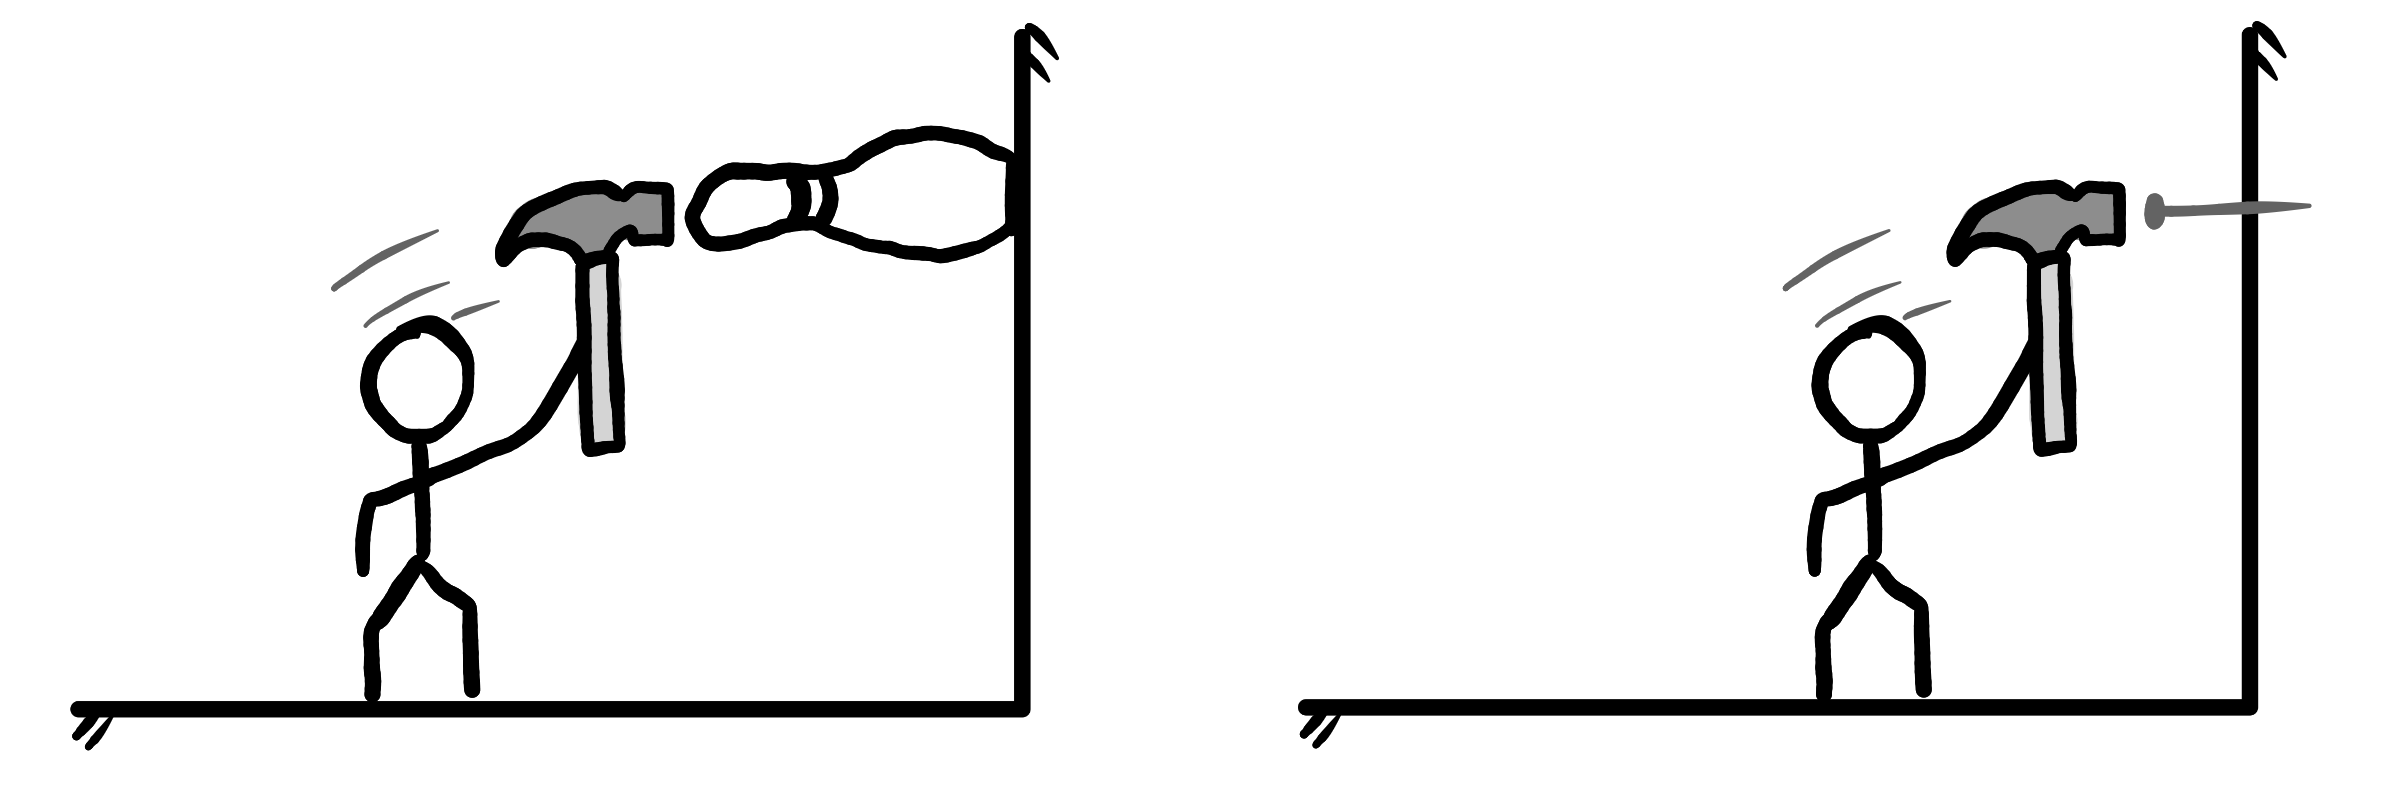
\includegraphics[width=0.6\linewidth]{imagensfluidos/definicaopressao.png}};
  \end{scope}
\end{tikzpicture}
\captionof{figure}{Uma mesma força $F$ da martelada aplicada em uma área menor -- no prego -- irá gerar um pressão muito maior.}
\label{fig_fluidos_definicaopressao}
} 
\vspace{0.3cm}




 A escolha de dividir pela área é intuitiva: quanto menor a área, mais concentrada fica a força, e maior é o efeito local: uma alta pressão pode perfurar uma parede, como mostra a Figura \ref{fig_fluidos_definicaopressao}. Já a mesma força, feita em uma área maior, digamos, um pino de boliche, gera uma pressão bem menor, e inviabiliza a perfuração, por exemplo.









\secgfe{Onde é usada}


A definição de pressão é a porta de entrada para o estudo dos fluidos. Em todas as equações desse capítulo o conceito de pressão irá aparecer, direta ou indiretamente.
 
% \begin{itemize}
%     \item \textbf{Lei de Stevin}, representada na Equação \eqref{eq_fluidos_leidestevin}: a pressão em um ponto submerso é calculada
%     somando a pressão na superfície à pressão exercida pela coluna de
%     líquido acima. Sem entender o que é pressão, é impossível construir ou compreender a Lei de Stevin.
 
%     \item \textbf{Princípio de Pascal}, representada na Equação \eqref{eq_fluidos_pascal}: que
%     afirma que uma variação de pressão aplicada a um fluido confinado
%     se transmite integralmente a todos os pontos~--- o coração da
%     prensa hidráulica.
 
%     \item \textbf{Empuxo} (seção \ref{sec:empuxo}): resultado da
%     diferença de pressão entre a face inferior e superior de um objeto
%     submerso. A força líquida que emerge dessa diferença é o que
%     chamamos de empuxo.
 
%     \item \textbf{Equação de Bernoulli} (seção \ref{sec:bernoulli}):
%     onde pressão, velocidade e altura de um fluido em movimento estão
%     relacionadas numa lei de conservação de energia.
% \end{itemize}
 
Fora da estudo dos fluidos, a pressão reaparece em \textbf{Termodinâmica} na lei dos gases ideais ($PV = nRT$), onde ela
é variável de estado fundamental. Em outros contextos, é comum encontrar problemas que combinam fluidos com equilíbrio estático~--- situações em que a condição $\sum \vec{F} = \vec{0}$ precisa ser aplicada a superfícies submetidas a pressões distintas.
 
No mundo real, a pressão está por toda parte: nos pneus de automóveis (pressão manométrica), nos equipamentos de mergulho, na meteorologia (pressão atmosférica e frentes de ar), nos freios hidráulicos, nas seringas e no funcionamento do coração humano.




\secgfe{Erros comuns}

Pontuaremos aqui as principais fontes de erros na aplicação da Equação \eqref{eq_fluidos_pressao}:

\begin{enumerate}
    \item [(i)] Usar a força total em vez da componente perpendicular à
superfície


Neste momento, convidamos o leitor a revisitar a Figura \ref{fig_dinamicanewton_planoinclinado03}, apresentada no contexto do estudo sobre a aceleração ao longo de um plano inclinado. Se um objeto de peso $P$ repousa sobre uma tal plano inclinado, de ângulo
$\theta$ com a horizontal, um erro comum é que o estudante calcule a pressão sobre a rampa
como $\mathcal{P} = P / A$, usando o peso total do bloco.\footnote{Usamos aqui uma grafia diferente para a pressão $\mathcal{P}$ apenas para não ser confundida com o peso $P$, que é a força geradora dessa pressão.}
 
O erro está em ignorar que pressão é definida como sendo a componente da
força \textbf{normal} (perpendicular) à superfície. O peso aponta
verticalmente para baixo, mas a superfície da rampa está inclinada.
A componente normal do peso sobre a rampa é $N=P_\perp = P\cos\theta$, como o leitor pode ver na Figura \ref{fig_dinamicanewton_planoinclinado03} (p. \pageref{fig_dinamicanewton_planoinclinado03}). Portanto, a pressão correta é
%
\begin{equation*}
    \mathcal{P}_{\text{rampa}} = \frac{P\cos\theta}{A}
\end{equation*}
%

 
% ---
 \item [(ii)] Esquecer de converter unidades de área.
 
Um erro comum é pegar uma área em cm$^2$ e substituir diretamente na Equação \eqref{eq_fluidos_pressao}, obtendo um resultado em
$\text{N}/\text{cm}^2$ sem perceber.
 
No SI, a unidade de pressão é o pascal (Pa): 

$$\SI{1}{Pa} = \dfrac{1 \text{N}}{\text{m}^2}.$$ 

Sendo assim, toda área deve estar em m$^2$ antes de aplicar a equação. 


Um outro erro comum é dividir por $10^2$ para converter cm$^2$ para m$^2.$ Este é o fator que converte cm em m -- as medidas lineares, e não as medidas quadráticas. De cm$^2$ para m$^2$ é preciso dividir por $(10^2)^2 = 10^4,$ como mostra a relação:

$$ 1 \text{cm} = 10^{-2} \text{m} \xrightarrow{\text{ elevando ao quadrado }} \boxed{1 \text{cm}^2 = 10^{-4} \text{m}^2.}$$

\end{enumerate}


Uma outra unidade comum de pressão é a de atm (atmosferas), definida de modo a ser unitária a pressão atmosférica na superfície da Terra, no nível do mar. Sendo assim, a pressão de 1 atm é igual à pressão exercida pela coluna de ar quando se está no nível do mar, e a conversão entre essas duas escalas é dada por

$$ \boxed{1 \text{ atm} \approx 1 \cdot 10^5 \text{ Pa.}}$$


\secgfe{Observações}

A pressão, apesar de ser definida com base em uma força -- que é uma grandeza vetorial -- trata-se de uma grandeza escalar. 


Embora a força que a origina seja vetorial, a pressão em si é uma grandeza escalar -- ela tem magnitude, mas não direção. Isso é possível porque a direção já foi incorporada na definição: é sempre a componente perpendicular à superfície considerada. Desse modo, a pressão em um ponto medirá a razão, naquele ponto, entre a componente da força perpendicular a uma superfície e a área da superfície em si. Tal valor não depende da orientação de tal superfície -- e é por isso que, em um ponto de um fluido, por exemplo, a pressão atua em todas as direções -- conforme veremos em breve.


\vspace{0.3cm}



\begin{exemplo}[Nível I]\label{exemplo_fluidos_pressaoex01}

Uma bailarina de massa $m=55$ kg executa um \emph{relevé} e apoia todo o seu peso na ponta de uma única sapatilha de ponta. A área de contato da ponta com o piso é de aproximadamente $A = \SI{1}{\centi\metre\squared}$. Calcule a pressão exercida sobre
o piso e compare com a pressão atmosférica $\mathcal{P}_{atm} \approx \SI{e5}{\pascal}$.
Adote $g = \SI{10}{\metre\per\second\squared}$.

\resolucao

O peso da bailarina concentra-se inteiramente na área $A$,
perpendicular ao piso horizontal. Pela definição de pressão:
 
\begin{equation}
    \mathcal{P} = \frac{F}{A} = \frac{mg}{A}
    \label{eq:pressao_bailarina} 
\end{equation}
 
Antes de substituir, convertemos a área para \si{\metre\squared}:
 
\begin{equation*}
    A = \SI{1}{\centi\metre\squared} = \SI{e-4}{\metre\squared}
\end{equation*}
 
Substituindo em \eqref{eq:pressao_bailarina}:
 
\begin{equation*}
    \mathcal{P} = \frac{55 \cdot 10}{10^{-4}}
    = \boxed{\SI{5{,}5e6}{\pascal} = \SI{5{,}5}{\mega\pascal}}
\end{equation*}
 
Comparando com a pressão atmosférica:
 
\begin{equation*}
    \frac{\mathcal{P}}{\mathcal{P}_{atm}}
    = \frac{5{,}5 \cdot 10^6}{10^5} = 55.
\end{equation*}
 
A pressão na ponta do sapatilha é \textbf{55 vezes} a pressão
atmosférica~--- resultado que rivaliza com equipamentos industriais
de médio porte. Uma força completamente ordinária, distribuída sobre
uma área extraordinariamente pequena, produz esse efeito. O assoalho
de madeira agradece quando a bailarina apoia os dois pés no solo.

\end{exemplo}






\vspace{0.3cm}






\begin{exemplo}[Nível II]\label{exemplo_fluidos_pressaoex02}

Um cilindro maciço homogêneo de raio $R$, altura $H$ e densidade $\rho$ está de pé sobre uma superfície horizontal.
 
\begin{enumerate}
    \item [a)] Expresse a pressão $\mathcal{P}$ que o cilindro exerce
          sobre a superfície em função de $\rho$, $H$ e $g$.
          O resultado deve surpreender o leitor.
    \item [b)] Dois cilindros idênticos são empilhados (um sobre o outro).
          Expresse a pressão na base do conjunto.
    \item [c)] Generalize: para uma pilha de $n$ cilindros idênticos,
          qual é a pressão na base?

\end{enumerate}

\resolucao

\textit{a)} A massa do cilindro é $m = \rho V = \rho \pi R^2 H$.
A área da base é $A = \pi R^2$. Portanto:
 
\begin{equation}
    \mathcal{P} = \frac{mg}{A}
               = \frac{\rho \pi R^2 H \cdot g}{\pi R^2}
               = \boxed{\rho g H}
    \label{eq:pressao_cilindro}
\end{equation}
 
O raio $R$ cancela completamente. A pressão que um cilindro
homogêneo exerce sobre sua base depende \textbf{apenas da sua
densidade e da sua altura}~--- não do seu raio, não da sua massa,
não da sua área de base. Um cilindro de alumínio fino como um
lápis e outro largo como uma coluna exercem a mesma pressão na
base, desde que tenham a mesma altura e a mesma densidade. Esse
resultado, que pode parecer contra-intuitivo à primeira vista,
é na verdade uma consequência direta e elegante da definição
$\mathcal{P} = F/A$: massa e área crescem juntos~--- ambos
proporcionais a $R^2$~--- e a razão entre eles independe de $R$. \\
 
\textit{b)} Com dois cilindros empilhados, a altura total é $2H$
e a base continua com área $\pi R^2$. Pelo resultado anterior, como a pressão depende apenas da densidade e da altura, teremos
 
\begin{equation*}
    \mathcal{P}_2 = \rho g (2H) = 2\,\rho g H,
\end{equation*}
 
\noindent ou seja, a pressão dobra. Cada cilindro adicionado contribui com a mesma parcela $\rho g H$. \\
 
\textit{c)} Para $n$ cilindros idênticos empilhados:
 
\begin{equation}
    \boxed{\mathcal{P}_n = n\,\rho g H.}
    \label{eq:pressao_n_cilindros}
\end{equation}
 
O leitor atento reconhecerá aqui o embrião da Lei de Stevin, dada pela Equação \eqref{eq_fluidos_leidestevin}, que será o nosso próximo objeto de estudo. A pressão cresce linearmente com a
``altura'' da coluna de material acima do ponto considerado. A transição de um sólido para um fluido não
altera esse resultado, conforme veremos em breve.
 
 

\end{exemplo}

\vspace{0.3cm}




\begin{exemplo}[Nível III]\label{exemplo_fluidos_pressaoex03}

Dois blocos homogêneos são empilhados sobre uma mesa horizontal. O
bloco inferior tem massa $M$ e base retangular de área $A$. O bloco
superior tem massa $m$ e base retangular de área $a$, com $a < A$.
O bloco superior está centrado sobre o inferior.
 
\begin{enumerate}
    \item [a)] Expresse a pressão $\mathcal{P}_1$ que o bloco superior
          exerce sobre o bloco inferior.
    \item [b)] Expresse a pressão $\mathcal{P}_2$ que o bloco inferior
          exerce sobre a mesa.
    \item [c)] Determine a condição sobre $m$, $M$, $a$ e $A$ para que
          $\mathcal{P}_1 > \mathcal{P}_2$~--- isto é, para que a
          pressão entre os dois blocos seja maior do que a pressão
          do conjunto sobre a mesa.
\end{enumerate}
 

\resolucao

\textit{a)} O único peso que age sobre o bloco inferior através da
interface de área $a$ é o peso do bloco superior, logo:
 
\begin{equation}
    \mathcal{P}_1 = \frac{mg}{a}
    \label{eq:p1_empilhados}
\end{equation}
 
\textit{b)} O bloco inferior apoia sobre a mesa o peso do sistema
completo, distribuído sobre sua própria base de área $A$:
 
\begin{equation}
    \mathcal{P}_2 = \frac{(M + m)\,g}{A}
    \label{eq:p2_empilhados}
\end{equation}
 
\textit{c)} Impondo $\mathcal{P}_1 > \mathcal{P}_2$ e usando
\eqref{eq:p1_empilhados} e \eqref{eq:p2_empilhados}:
 
\begin{equation*}
    \frac{mg}{a} > \frac{(M + m)\,g}{A}
\end{equation*}
 
Cancelando $g > 0$ e desenvolvendo, teremos:
 
\begin{equation*}
    mA > (M + m)\,a
    \implies
    mA > Ma + ma
    \implies
    m(A - a) > Ma
\end{equation*}
 
Portanto a condição é:
 
\begin{equation}
    \boxed{\frac{m}{M} > \frac{a}{A - a}}
    \label{eq:condicao_empilhados}
\end{equation}
 
O membro direito de \eqref{eq:condicao_empilhados}
é a razão entre a área de contato entre os blocos ($a$) e a área
``livre'' da base do bloco inferior ($A - a$). Convém analisar tal expressão em casos extremos, que tornam o significado físico mais intuitivo. \\

\textbf{Caso 1: base superior muito pequena ($a \ll A$)} \\
Quando $a$ é muito menor que $A$, o denominador $A - a \approx A$,
e a condição se torna $m/M > a/A \approx 0$. Ela é satisfeita para
qualquer par de massas positivas. Faz sentido: o bloco superior
concentra todo o seu peso numa interface minúscula de área $a$,
gerando uma pressão $\mathcal{P}_1 = mg/a$ muito alta. A mesa, por
outro lado, sustenta os dois blocos espalhados sobre a área grande
$A$, diluindo $\mathcal{P}_2$. Nesse regime, $\mathcal{P}_1 >
\mathcal{P}_2$ quase inevitavelmente. \\
 
\textbf{Caso 2: base superior quase igual à inferior ($a \to A$).} \\
Agora $A - a \to 0$, e o membro direito $a/(A - a) \to \infty$.
A condição nunca é satisfeita, independentemente de quão maior
seja $m$ em relação a $M$. Faz sentido: se os dois blocos têm bases
iguais, a interface entre eles tem a mesma área que a base sobre a
mesa~--- mas carrega apenas o peso $mg$, enquanto a mesa carrega
$mg + Mg$. A pressão na mesa é necessariamente maior.\\
 
\textbf{Caso intermediário: quando as pressões se igualam.} \\
A igualdade $m/M = a/(A - a)$ marca exatamente o ponto em que
$\mathcal{P}_1 = \mathcal{P}_2$. Por exemplo, se $a = A/2$ (bloco
superior ocupa metade da base inferior), a condição de igualdade
exige $m/M = 1$, ou seja, $m = M$. Se o bloco de cima for mais
pesado que o de baixo, a pressão na interface supera a pressão na
mesa; se for mais leve, ocorre o contrário. \\
 
Em suma, a condição \eqref{eq:condicao_empilhados}
é um balanço entre dois efeitos opostos: a concentração de carga
causada pela área pequena $a$ (que eleva $\mathcal{P}_1$) e a
diluição de carga causada pela área grande $A$ (que abaixa
$\mathcal{P}_2$). O que determina qual efeito vence não é a massa
isolada nem a área isolada~--- é a razão entre elas, comparada
simultaneamente para os dois blocos.
 


\end{exemplo}

\vspace{0.3cm}






\begin{secnivel}[Lei de Stevin]{I}{Lei de Stevin}
 

  \eqLdois{dem}{eq_fluidos_leidestevin}{\Delta p =\rho g\Delta h }
  
\end{secnivel}






\secgfe{De onde vem}

A Equação \eqref{eq_fluidos_leidestevin} serve para calcular a diferença de pressão $\Delta p$ entre dois pontos de um fluido de densidade $\rho$, separados por um desnível vertical $\Delta h$, em uma região do espaço em que a gravidade é $g.$

Considere, para tanto, um aquário preenchido com um fluido de densidade $\rho$, em equilíbrio hidrostático. Imagine que façamos um recorte para analisar uma certa porção cilíndrica deste fluido, de altura $\Delta h$, como mostra a Figura \ref{fig_fluidos_stevinproof}.



\vspace{0.3cm}
{
\centering
\begin{tikzpicture}
  \begin{scope}[blend mode=multiply]
    \node {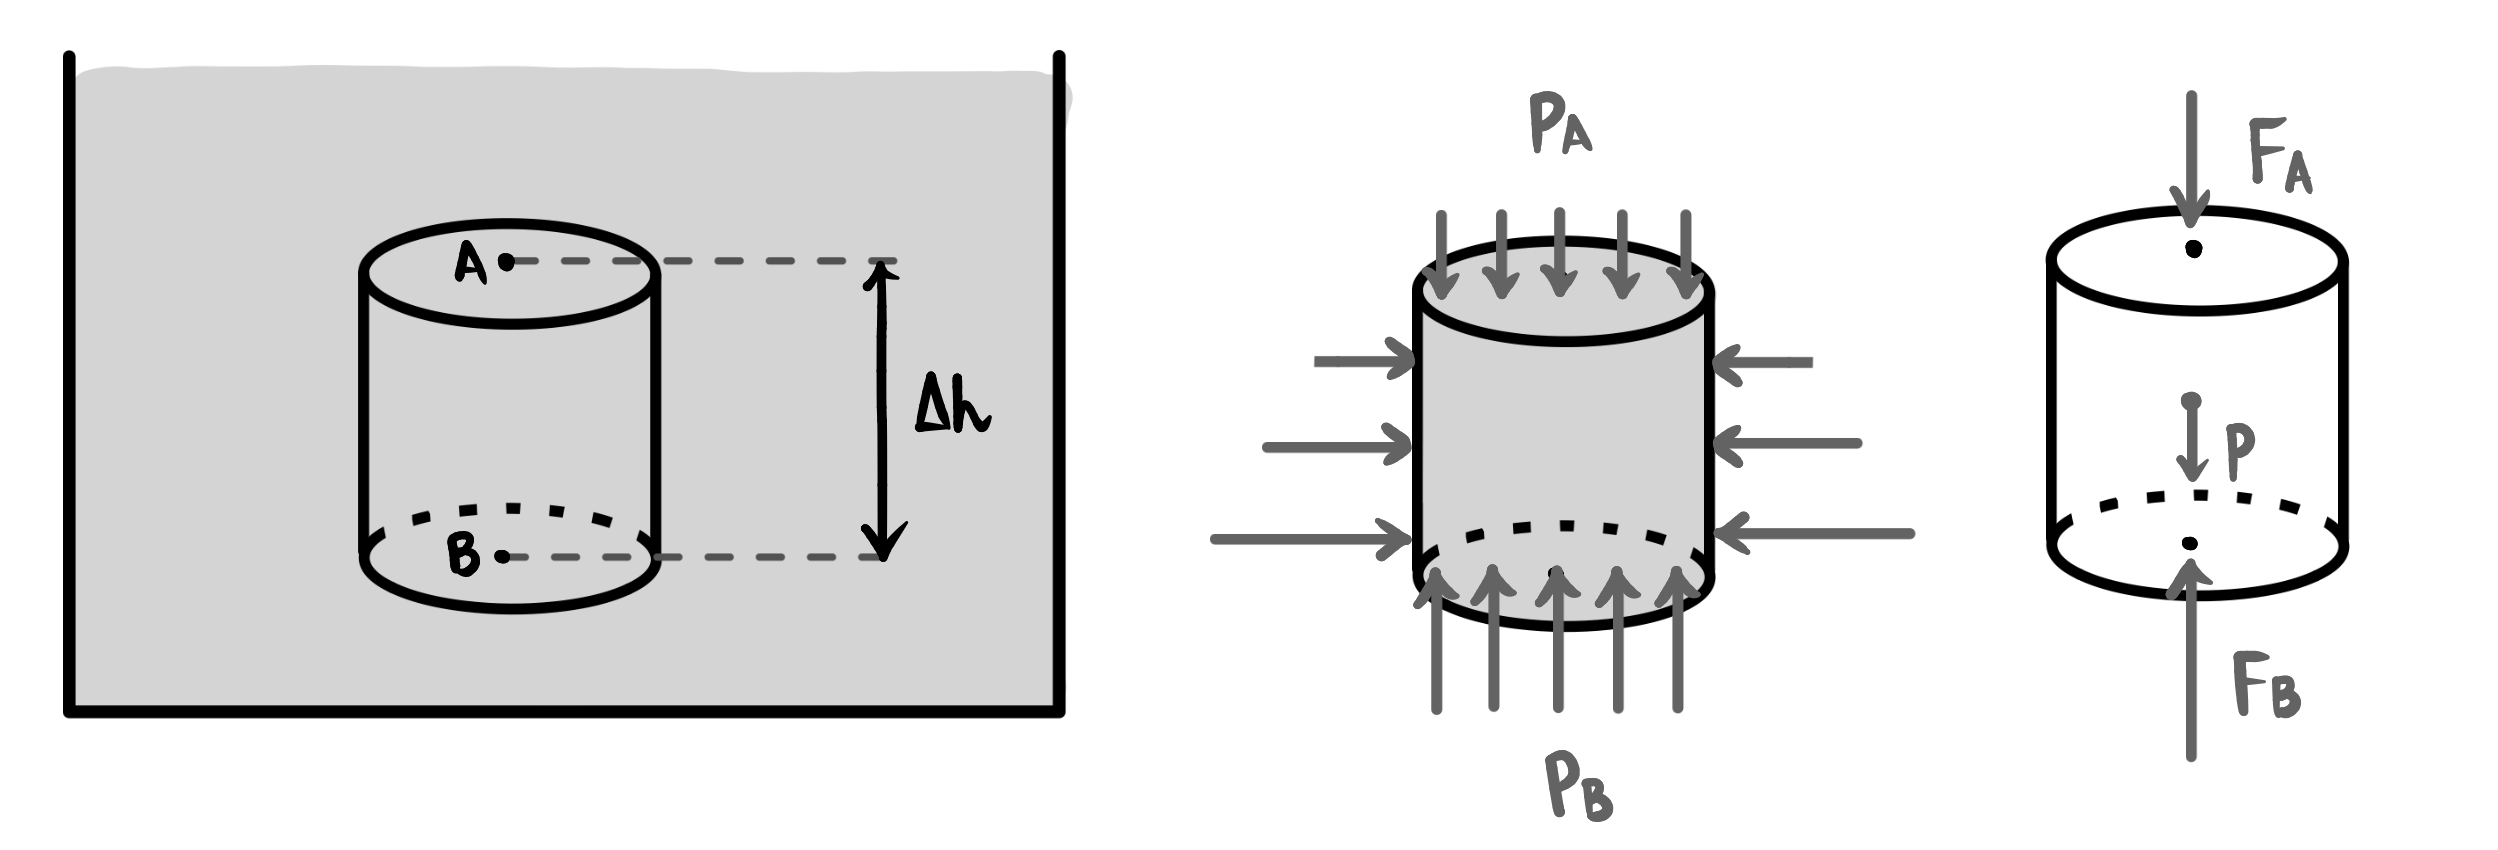
\includegraphics[width=0.9\linewidth]{imagensfluidos/stevinproof.png}};
  \end{scope}
\end{tikzpicture}
\captionof{figure}{Porção cilíndrica de fluido em equilíbrio hidrostático.}
\label{fig_fluidos_stevinproof}
} 
\vspace{0.3cm}

Ora, como se trata de hidrostática, qualquer porção do fluido -- e o fluido como um todo -- está em equilíbrio, o que vale, em particular, para o pequeno cilindro destacado.

A segunda imagem da figura mostra a distribuição de pressões no cilindro ao longo de seu comprimento: ele é pressionado de todos os lados. Por simetria, as pressões horizontais deverão se anular -- é isso que garantirá o equilíbrio da porção cilíndrica de fluido na horizontal, isto é, que $\sum F_x = 0.$ Em um primeiro momento, o leitor poderia pensar também que a pressão em $A$ deveria ser igual à pressão em $B,$ para que haja equilíbrio na vertical. Contudo, ao longo dessa direção, há uma força a mais: o peso dessa porção de fluido.

A última imagem mostra o diagrama de forças na vertical que atua neste cilindro: ele é empurrado para baixo com uma força $F_A$ (devido à pressão $P_A$ em sua face superior); além disso, há também sua força peso, que o puxa para baixo. Para anular essas duas, só restou a força vertical $F_B$, devido à pressão $P_B$ na face inferior do cilindro. Dessa análise qualitativa já podemos concluir que $P_B > P_A,$ isto é, nos pontos de maior profundidade a pressão deve ser maior -- porque ela deve gerar uma força capaz de sustentar tanto a pressão que empurra o cilindro para baixo quanto seu próprio peso.

Escrevendo isso de forma matemática, teremos (não confundir o peso $P$ do cilindro com alguma pressão):

$$ \sum F_y = 0 \implies F_B = F_A + P \implies P_B \cdot A = P_A \cdot A + mg, $$

\noindent em que $A$ é a área da base do cilindro, ao longo da qual a pressão atua. Usamos, com isso, a definição de pressão dada pela Equação \eqref{eq_fluidos_pressao}. Sendo $\rho$ a densidade do fluido, podemos escrever para a porção cilíndrica de fluido:

$$ \rho = \dfrac{m}{V} = \dfrac{m}{A\cdot \Delta h} \implies m = \rho \cdot A \cdot \Delta h,$$

\noindent de modo que a equação anterior se torna

$$ P_B \cdot \cancel A = P_A \cdot \cancel A+  \rho \cdot \cancel A \cdot \Delta  h \cdot g,$$

\noindent e, como o fator área simplifica em todos os termos, ficamos com 

$$ P_B = P_A + \rho g \Delta h,$$

\noindent ou seja, a pressão em um ponto $B,$ de maior profundidade, é maior do que a pressão em um ponto $A,$ em um nível acima, como previsto. Ela é maior exatamente de $\rho g h,$ de modo que poderíamos escrever a relação acima como

$$ P_B - P_A = \Delta p = \rho g \Delta h,$$

\noindent que vem a ser exatamente a forma como apresentamos a Equação \eqref{eq_fluidos_leidestevin}. 

Perceba, portanto, que pressão extra gerada no ponto $B$, devido ao peso da coluna de fluido que está acima de $B$, depende exclusivamente da altura de fluido acima de tal ponto -- é isso que significa a simplificação do fator área no desenvolvimento de tal equação.

O fato de a área se simplificar é tão importante que merece um destaque a parte. Considere a Figura \ref{fig_fluidos_leistevinarnold}, que mostra dois indivíduos, de mesma altura, no fundo do mar. Um deles possui a cabeça mais achatada, no formato de uma bola de futebol americano. 


\vspace{0.3cm}
{
\centering
\begin{tikzpicture}
  \begin{scope}[blend mode=multiply]
    \node {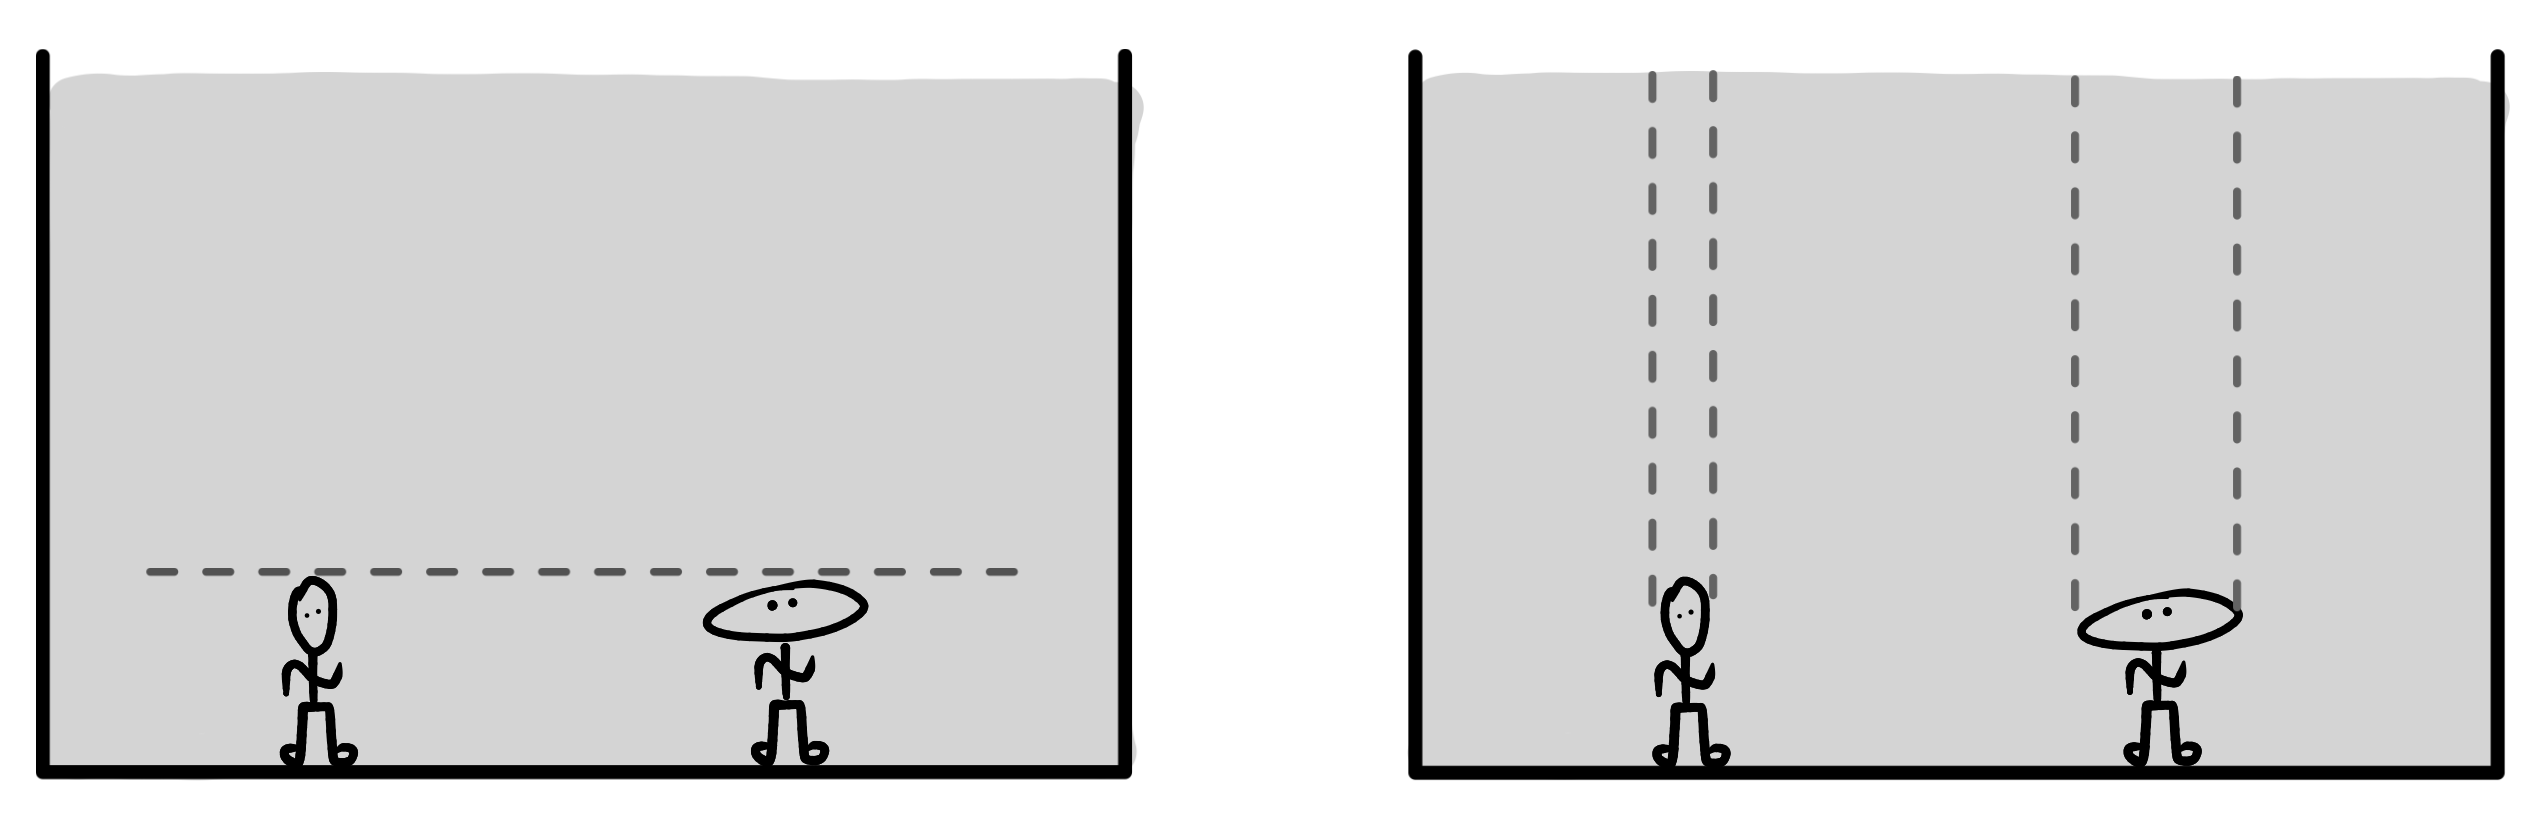
\includegraphics[width=0.8\linewidth]{imagensfluidos/leistevinarnold.png}};
  \end{scope}
\end{tikzpicture}
\captionof{figure}{A pressão sob a cabeça dos dois indivíduos é a mesma, ainda que o peso da coluna de água sob a cabeça deles seja diferente.}
\label{fig_fluidos_leistevinarnold}
} 
\vspace{0.3cm}

Em um primeiro momento, como mostra a segunda imagem, poderíamos pensar que a pressão da coluna de água sob a cabeça do indivíduo de cabeça achatada é maior: a coluna de água sob sua cabeça, apesar de ter a mesma altura, possui maior área, de modo que o volume é maior. Isso está correto: o peso da coluna de água sob a cabeça de tal indivíduo é, de fato, maior do que o peso da coluna de água sob a cabeça do indivíduo cuja calota craniana é regular. Isso quer dizer que a força que comprime a cabeça do indivíduo de crânio achatado é maior do que a daquele outro indivíduo de cabeça regular, e até aqui está tudo certo.

O erro comum é achar que, por isso, a pressão sobre a cabeça dos indivíduos é diferente, mas elas acabam sendo iguais. Isso porque a pressão mede a força por unidade de área, e o peso da coluna de água sob a crânio do indivíduo de cabeça achatada é maior justamente porque a área da base de tal coluna é maior. Ou seja, digamos que o indivíduo de crânio normal tenha uma área $A$ da seção transversal de sua cabeça. Seja $F$ a força peso da coluna de água sob a sua cabeça.

Se o nosso camarada de cabeça achatada tiver uma área de seção transversal craniana três vezes maior, isto é, $3A,$ isso implicará que a coluna de água sob a sua cabeça terá o triplo do peso, ou seja, a força que o comprime será $3F.$ Fazendo a razão entre essas duas, o fator $3$ desaparece -- é isso que significa o fator área simplificar no nosso desenvolvimento -- de modo que as pressões sob as duas cabeças são iguais:

$$ P_1 = \dfrac{F}{A} \quad \text{ e } \quad P_2 = \dfrac{\cancel 3F}{\cancel 3A} =  \dfrac{F}{A} = P_1 .$$

Ou seja, pontos que estejam a um mesmo nível de profundidade $h$ suportarão a mesma pressão, independente da área de contato do objeto imerso nesse ponto.





\secgfe{Onde é usada}



Tal equação se aplica para entender o tipo de pressão que, por exemplo, um submarino estará submetido, o que é necessário na hora de projetar sua estrutura. Considerando a densidade da água como sendo $\rho= 1$g/cm$^3$ = $10^3$ kg/m$^3$, podemos calcular, por exemplo, a pressão gerada por uma coluna de 10 metros de água:

$$ P = \rho g h = 10^3 \cdot 10 \cdot 10 = 1 \cdot 10^5 \text{ Pa} \approx 1 \text{ atm.}$$

Este talvez seja um fato conhecido pelo leitor: a cada 10 metros de imersão no mar a pressão aumenta de 1 atm: esse é um resultado que segue diretamente da aplicação da Equação \eqref{eq_fluidos_leidestevin}. Um submarino militar costuma navegar a profundidades de 400 metros, o que implica ter que sustentar uma pressão de 40 atm devido ao peso da coluna de água que está acima dele. Note que essa é uma pressão 40 vezes superior à pressão sentida na atmosfera, no nível do mar, de modo que precisa ser levada em consideração ao projetar a estrutura e a rigidez de um submarino.

Tal equação também se aplica em contextos residenciais: estando a caixa d'água no topo de um prédio, os apartamentos mais baixos (os primeiros andares) terão acesso a uma maior pressão da água nos chuveiros e torneiras, haja vista que a coluna de água é mais alta sob esses andares.

Um outro contexto de importante aplicação para se medir o nível de água em reservatórios é o dos vasos comunicantes. Considere, por exemplo, um sistema de dois vasos de diferentes formatos geométricos que são preenchidos pelo mesmo fluido, podendo se comunicar na parte inferior, como mostra a Figura \ref{fig_fluidos_vasoscomunicantes}.

\vspace{0.3cm}
{
\centering
\begin{tikzpicture}
  \begin{scope}[blend mode=multiply]
    \node {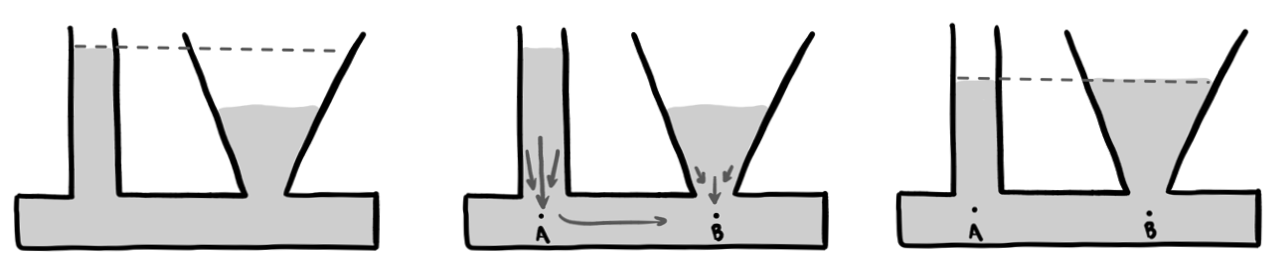
\includegraphics[width=0.8\linewidth]{imagensfluidos/vasoscomunicantes.png}};
  \end{scope}
\end{tikzpicture}
\captionof{figure}{Princípio dos vasos comunicantes.}
\label{fig_fluidos_vasoscomunicantes}
} 
\vspace{0.3cm}


Suponha que, na situação de equilíbrio estático, o sistema fique como aparece na primeira imagem. Ora, neste caso, sabemos que a pressão $P_A$ no ponto $A$, dada por $P_A = \rho g h_{A}$, será maior do que a pressão no fundo do vaso $B$, dada por $P_B = \rho g h_{B}$.\footnote{Sendo o mesmo fluido e submetidos à mesma gravidade $g$, a pressão em $A$ é maior que em $B$ haja vista que $h_A > h_B.$} Logo, como mostra a segunda imagem, o fato de existir uma diferença de pressão significa que o sistema não está em equilíbrio: a pressão abaixo do vaso $A,$ empurrando o fluido para baixo, é maior do que a pressão abaixo do vaso $B$, que também empurra o fluido para baixo. 

Desse modo, a diferença de pressão gera um fluxo de fluido -- a situação, portanto, não é de hidrostática -- até que se alcance o equilíbrio, o que ocorrerá justamente quando não houver diferença de pressão, ou seja, quando os níveis de fluido nos dois vasos for exatamente o mesmo, de modo a não haver diferença de pressão no fundos dos recipientes. A última imagem mostra esta configuração de equilíbrio.

Um sistema como esse pode ser usado para aferir o nível de água em um reservatório. O medidor de nível mais simples possível é um tubo transparente conectado lateralmente a um reservatório opaco. O líquido sobe no tubo até a mesma altura que no reservatório -- vasos comunicantes em sua forma mais pura -- o que nos permite saber o nível de água dentro do reservatório sem precisar vê-lo por dentro, diretamente.




\secgfe{Erros comuns}

O erro mais comum é fazer uma confusão em relação às unidades de medida. Lembre-se que, para obter a pressão em unidades do SI, isto é, em Pascal (Pa), é preciso que a densidade $\rho$ seja expressa em kg/m$^3$, a gravidade $g$ em m/s$^2$ e o desnível $\Delta h$ em metros. 

Além disso, um erro de principiante é considerar a altura em relação ao fundo, e não ao nível superior da água. Ou seja, na situação da Figura \ref{fig_fluidos_stevinerro}, seria usar o valor de 1m como $\Delta h,$ enquanto o correto é o valor de 3m. Lembre que a pressão é relativa ao peso da coluna de líquido que está \textbf{acima} daquele ponto, de modo que o desnível vertical considerado é sempre em relação à superfície do líquido.


\vspace{0.3cm}
{
\centering
\begin{tikzpicture}
  \begin{scope}[blend mode=multiply]
    \node {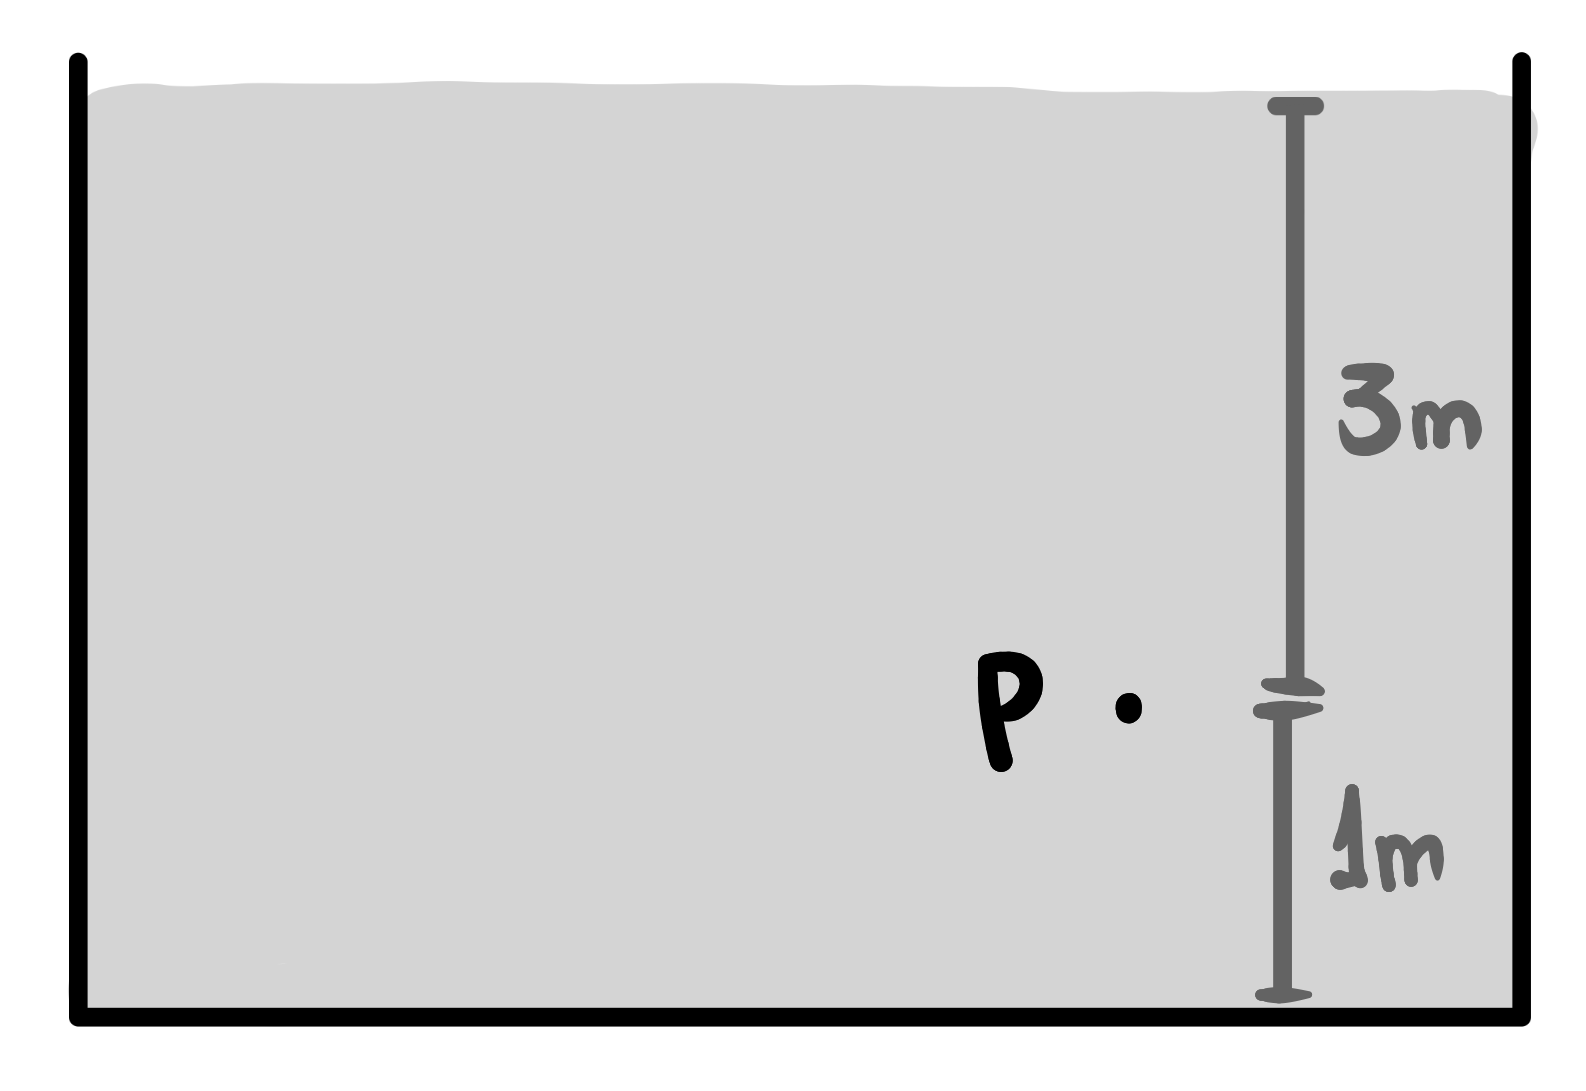
\includegraphics[width=0.3\linewidth]{imagensfluidos/stevinerro.png}};
  \end{scope}
\end{tikzpicture}
\captionof{figure}{A pressão em um ponto é devido à coluna de líquido que está acima desse ponto, e não abaixo dele.}
\label{fig_fluidos_stevinerro}
} 
\vspace{0.3cm}



Um erro bastante comum também é o de considerar que dois pontos em um mesmo nível de um fluido em repouso sempre terão a mesma pressão. Isso só é verdade para um \emph{mesmo líquido}: como a pressão é $P = \rho g h,$ se $\rho$ é o mesmo -- mesmo fluido -- então, dado um mesmo $h$ -- mesmo nível -- a pressão deve ser igual (dado que $g$ é o mesmo nos dois pontos). Contudo, se tivermos fluidos diferentes, serão necessárias alturas diferentes $h$ de colunas destes fluidos para gerar a mesma pressão $P$, haja vista que suas densidades $\rho$ serão diferentes.

Dado dois fluidos $A$ e $B,$ de densidades $\rho_A$ e $\rho_B,$, é possível, inclusive, computar a razão entre as alturas das colunas desses fluidos que geram a mesma pressão:

$$ P_A = P_B \implies \rho_A \cancel g h_A = \rho_B \cancel g h_B \implies \boxed{ \dfrac{h_A}{h_B} = \dfrac{\rho_B}{\rho_A}.}  $$

Note que:

\begin{itemize}
    \item [(i)] $ \rho_A = \rho_B \implies h_A = h_B$. 

    Ou seja, se o fluido é o mesmo (mesma densidade), dois pontos de mesma pressão estão no mesmo nível: $h_A=h_B.$ Ou, caso o leitor prefira, dois pontos em um mesmo nível -- mesmo $h$ -- suportam a mesma pressão.

     \item [(ii)] Fluidos mais densos exigem uma coluna de líquido de altura menor para gerar a mesma pressão. A expressão mostra que a razão entre as alturas é o inverso da razão entre as densidades: um fluido duas vezes mais denso precisa de metade da altura de coluna para gerar a mesma pressão que um fluido que tenha metade da sua densidade:

\[
P=
\underbrace{(2\rho)\cdot g \cdot h}_{\substack{\text{densidade }2\rho\\ \text{altura }h}}
=
\underbrace{\rho\cdot g \cdot(2 h)}_{\substack{\text{densidade }\rho\\ \text{altura }2h}}
\]


\end{itemize}

O segundo exemplo dessa seção trata justamente deste caso.




\secgfe{Observações}

A  Equação \eqref{eq_fluidos_leidestevin} calcula a diferença de pressão em um fluido qualquer de densidade constante $\rho$.
 Fluidos são tanto líquidos como gases, porém a equação em questão é particularmente útil para o cálculo de pressão em líquidos, haja vista que, para gases, como sua densidade é muito pequena, a diferença de pressão entre dois pontos próximos é praticamente nula. Considere, por exemplo, dois pontos afastados verticalmente de 10 metros na superfície da Terra. Se tais pontos estão dentro de um aquário com água, a diferença de pressão entre eles será

 $$ \Delta p = \rho_{H_2 O} \cdot g \cdot \Delta h  = 10^3 \text{ kg/m}^3 \cdot 10 \text{m/s}^2 \cdot 10 \text{m} = 1 \cdot 10^5 \text{ Pa} \approx 1 \text{ atm.}$$

 Já se os dois pontos em questão estiverem imersos no ar atmosférico, a diferença de pressão entre eles será de 

 $$ \Delta p = \rho_\text{AR} \cdot g \cdot \Delta h  = 1.2 \text{ kg/m}^3 \cdot 10 \text{m/s}^2 \cdot 10 \text{m} = 1.2 \cdot 10^2 \text{ Pa} \approx 0.0012 \text{ atm.}$$

 Ou seja, no caso do ar, a diferença de pressão entre os mesmos dois pontos é cerca de mil vezes menor. Se estivermos em um local no qual a pressão atmosférica é de $1$ atm, a diferença de pressão acima representa uma variação de apenas 0.12\%, de modo que é razoável supor que, para gases, a sua pressão é aproximadamente constante e a Equação \eqref{eq_fluidos_leidestevin} não se aplica.\footnote{É importante ficar claro que, em teoria, a equação se aplica sim. Contudo, como vimos, ao aplicá-la, os valores de diferença de pressão gerados são desprezíveis.}

 É claro que, para valores de $\Delta h$ muito altos, como por exemplo da ordem de 1 km, ou de algumas dezenas de quilômetros, a Equação \eqref{eq_fluidos_leidestevin} forneceria uma diferença de pressão significativa para gases: mesmo estes tendo uma densidade muito baixa, um alto desnível $\Delta h$ pode compensar isso, gerando variações relevantes de pressão. Contudo, ao variar muito a altitude, isto é, para $\Delta h$ da ordem de algumas dezenas de quilômetros, a densidade do ar também varia significativamente, de modo que a Equação \eqref{eq_fluidos_leidestevin} não pode ser aplicada. Tal equação parte da premissa que a densidade $\rho$ do fluido é constante.


\vspace{0.3cm}



\begin{exemplo}[Nível I]\label{exemplo_fluidos_stevinex01}

Uma piscina está preenchida com água até uma altura $h = \SI{2}{\metre}$.
A pressão na superfície é a atmosférica, $P_0 = \SI{e5}{\pascal}$.
Calcule a pressão absoluta no fundo da piscina. Adote
$\rho_{\!agua} = \SI{e3}{\kilo\gram\per\metre\cubed}$ e
$g = \SI{10}{\metre\per\second\squared}$.

\resolucao

Aplicando diretamente a Lei de Stevin, com $h$ medido a partir da
superfície livre até o fundo:
 
\begin{equation*}
    P = P_0 + \rho g h
    = 10^5 + 10^3 \cdot 10 \cdot 2
    = 10^5 + 2 \cdot 10^4
\end{equation*}
 
\begin{equation*}
    \boxed{P = 1{,}2 \cdot 10^5\,\si{\pascal} = 1{,}2\,\text{atm.}}
\end{equation*}
 
A coluna de água de \SI{2}{\metre} acrescenta apenas $0{,}2\,\text{atm}$
à pressão atmosférica~--- uma parcela modesta. Isso ajuda a entender
por que nadar em piscinas razoavelmente fundas não é desconfortável:
a pressão extra sobre os tímpanos equivale a apenas um quinto de uma
atmosfera.

\end{exemplo}


\vspace{0.3cm}






\begin{exemplo}[Nível II]\label{exemplo_fluidos_stevinex02}

Um tubo em~U contém, no lado esquerdo, uma coluna de mercúrio de densidade
$\rho_{m}$ e altura $h_1$ acima da interface mercúrio-água. O lado direito contém apenas água de densidade $\rho_{a}$, como mostra a Figura \ref{fig_fluidos_tuboU1}.

\vspace{0.3cm}
{
\centering
\begin{tikzpicture}
  \begin{scope}[blend mode=multiply]
    \node {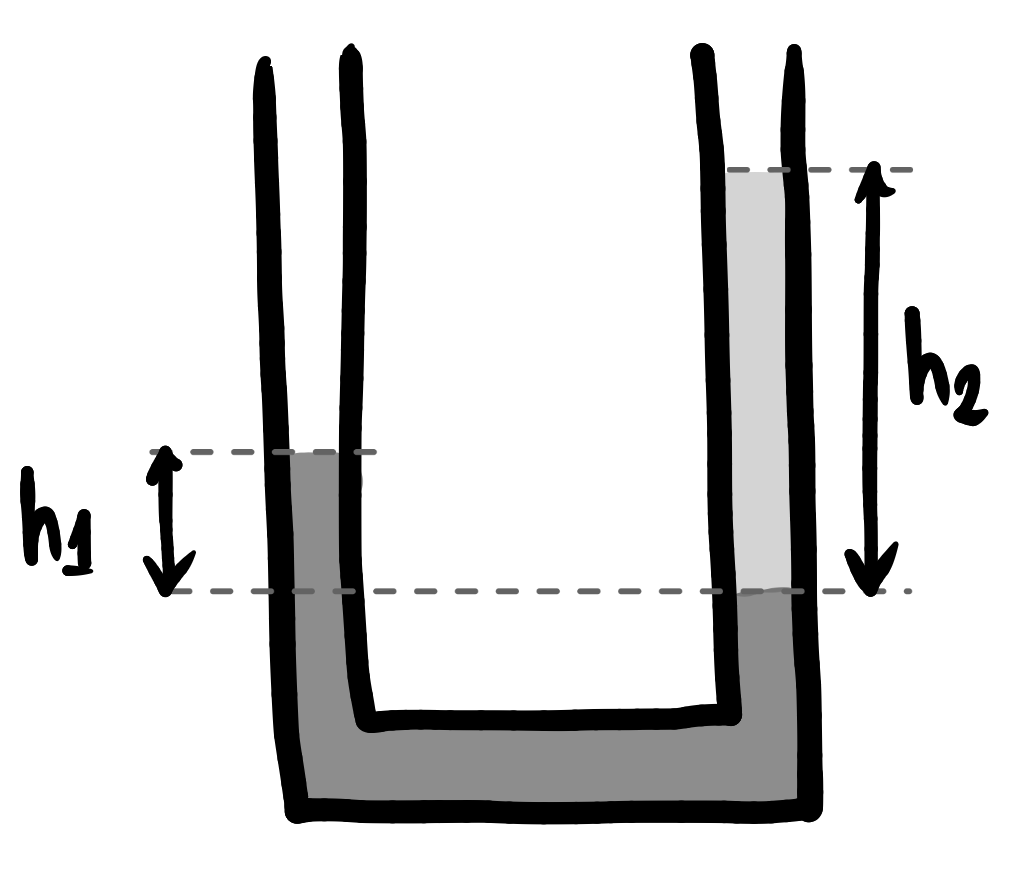
\includegraphics[width=0.3\linewidth]{imagensfluidos/tuboU1.png}};
  \end{scope}
\end{tikzpicture}
\captionof{figure}{}
\label{fig_fluidos_tuboU1}
} 
\vspace{0.3cm}


Calcule a densidade $\rho_m$ do mercúrio.
Adote $g$ como a aceleração da gravidade local e
$\rho_a = 1 \text{ g/cm}^3$,
$h_1 = \SI{5}{\centi\metre}$ e $h_2 = \SI{68}{\centi\metre}.$

\resolucao

Quando misturamos dois líquidos imiscíveis em um tubo em $U,$ como na situação da Figura \ref{fig_fluidos_tuboU1}, temos em mão um experimento que nos permite, por exemplo, determinar a densidade de um desses líquidos, apenas medindo os parâmetros $h_1$ e $h_2,$ desde que conhecida a densidade do outro líquido, como veremos.

O raciocínio executado aqui é análogo ao que fizemos na situação da Figura \ref{fig_fluidos_vasoscomunicantes}, sobre os vasos comunicantes. 



\vspace{0.3cm}
{
\centering
\begin{tikzpicture}
  \begin{scope}[blend mode=multiply]
    \node {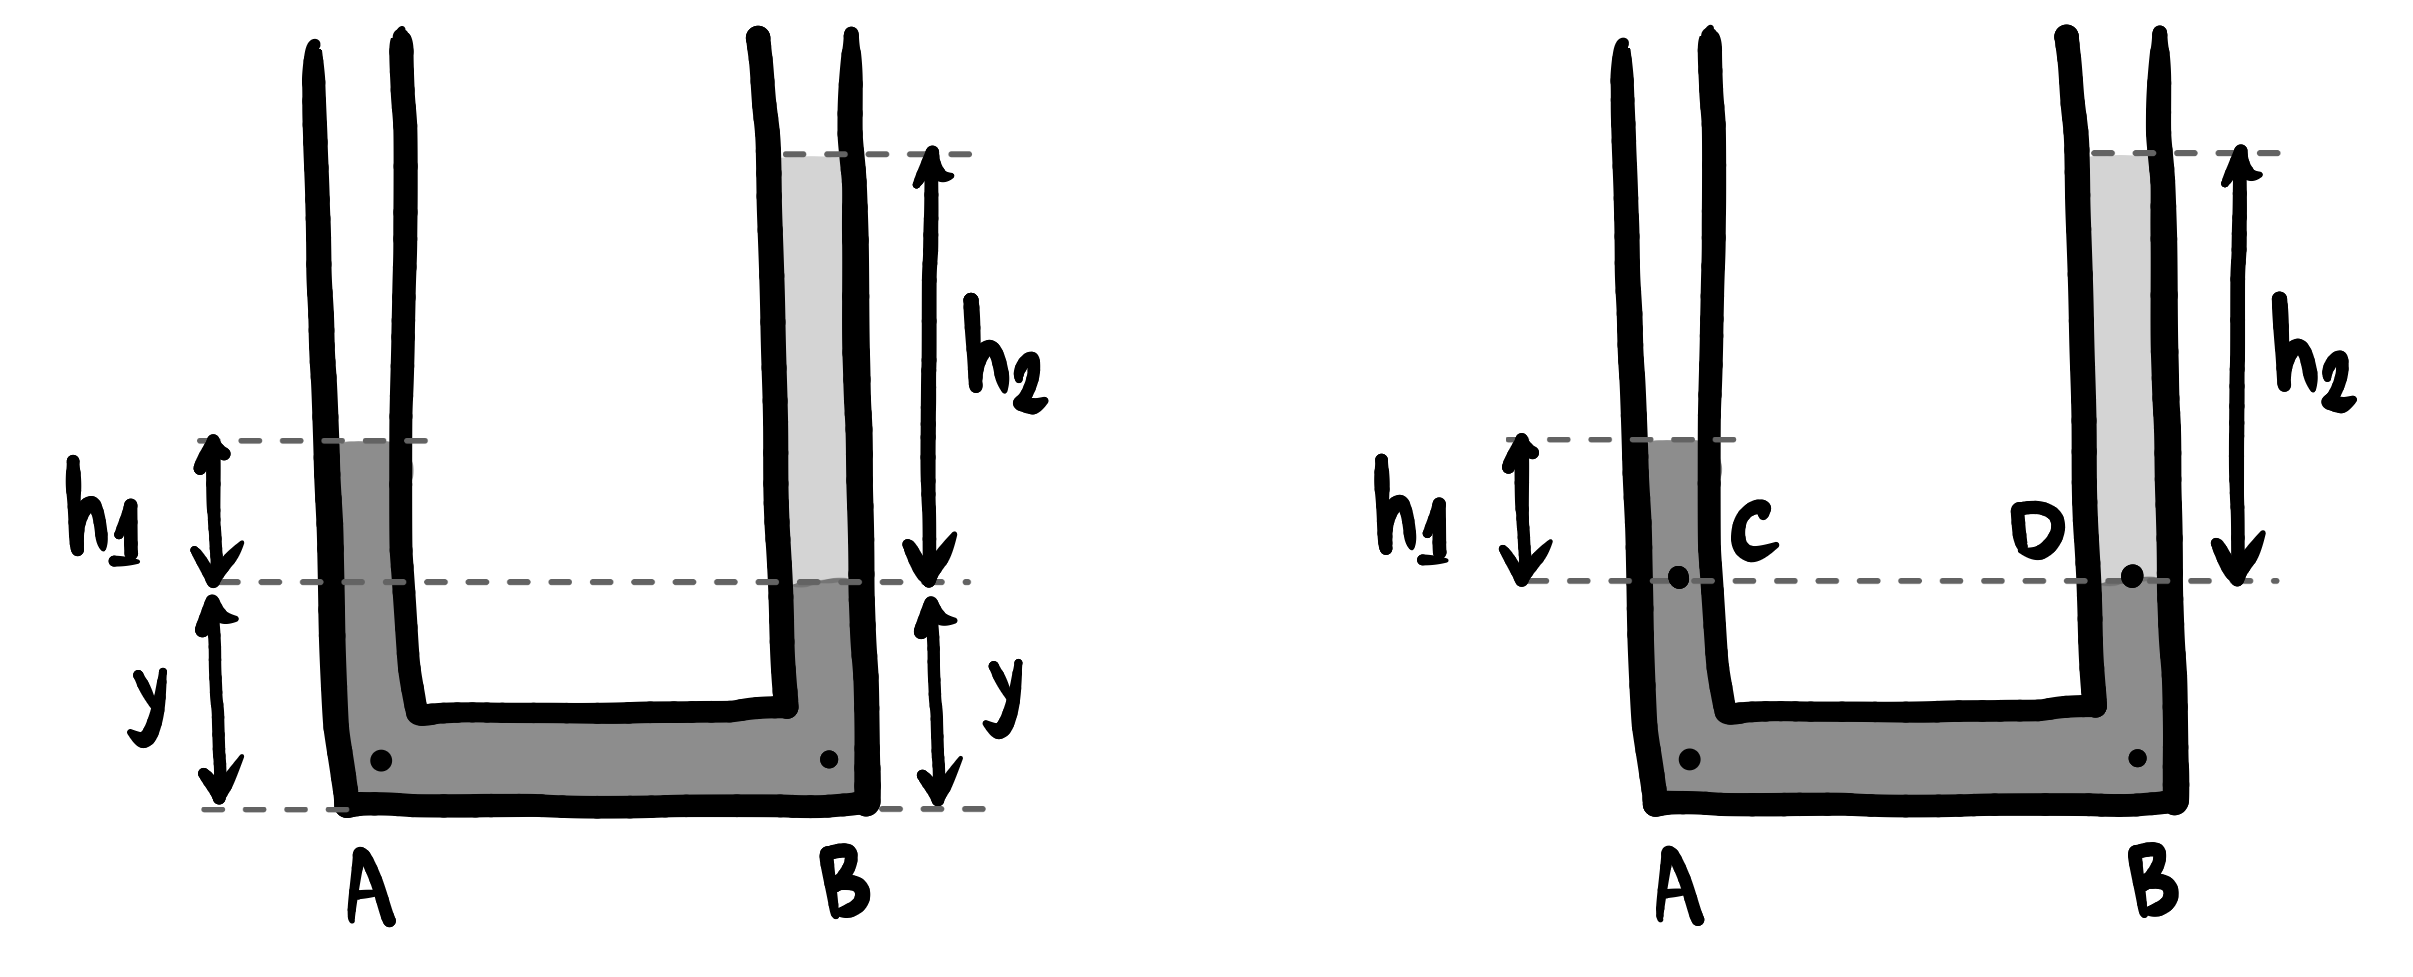
\includegraphics[width=0.7\linewidth]{imagensfluidos/tuboU2.png}};
  \end{scope}
\end{tikzpicture}
\captionof{figure}{O equilíbrio mecânico dos fluidos exige que a pressão no fundo de cada braço seja a mesma: $P_A=P_B.$}
\label{fig_fluidos_tuboU2}
} 
\vspace{0.3cm}


Como mostra a primeira Figura \ref{fig_fluidos_tuboU2}, se o sistema está em equilíbrio, então não pode haver diferença de pressão no fundo do recipiente, isto, é, precisamos que $P_A = P_B.$ Se os tubos estão abertos para a atmosfera, que possui uma pressão local $P_0,$ então segue que

$$ P_A = P_B \implies \cancel {P_0 } + \rho_m gh_1+  \cancel {\rho_m gy } = \cancel {P_0 } + \rho_agh_2 + \cancel {\rho_m gy }, $$

\noindent ou seja isso exige que 

\begin{equation}
    \rho_m gh_1 =\rho_agh_2.
    \label{eq_fluidos_tuboU}
\end{equation}


Observando a segunda imagem da Figura \ref{fig_fluidos_tuboU2}, isso diz que $P_C = P_D.$ Perceba que tal equação é bastante natural e poderia ter sido escrita diretamente, uma vez que, para exigir que a pressão seja a mesma no fundo dos braços, ou seja, em $A$ e $B$, a pressão atmosférica $P_0$ será irrelevante, uma vez que ela atua igualmente dos dois lados -- é por isso que tal termo se cancela na equação. 

Além disso, a pressão devido à coluna de mercúrio de altura $y$ também é pouco relevante, uma vez que ela também atua igualmente dos dois lados -- também é por isso que tal termo se cancela. Assim, para garantir a igualdade de pressões em $A$ e $B$ basta garantir que a coluna de mercúrio acima da superfície de interface mercúrio-água (a coluna de altura $h_1$) exerça a mesma pressão que a coluna de água acima de tal interface, isto é, a coluna de água de altura $h_2.$



Naturalmente, sendo menos densa que o mercúrio, a água precisará de uma maior altura para exercer a mesma pressão, e é por isso que o tubo fica em equilíbrio com níveis diferentes dos dois lados: fluidos de densidades diferentes precisarão de alturas diferentes de suas colunas para gerarem a mesma pressão. Desenvolvendo a Equação \eqref{eq_fluidos_tuboU} teremos:

$$ \rho_m = \dfrac{h_2}{h_1} \rho_a = \dfrac{68}{5} \cdot 1 \text{ g/cm}^3 \implies \boxed{\rho_m =13.6 \text{ g/cm}^3.} $$

 


\end{exemplo}


\vspace{0.3cm}






\begin{exemplo}[Nível III]\label{exemplo_fluidos_stevinex03}


Uma barragem retém água de densidade $\rho$ até uma altura $H$ acima
de sua base. A parede da barragem é vertical, plana e tem largura $L$
(perpendicular ao plano do problema). A pressão na superfície da água
é $P_0$.
 
\begin{enumerate}
    \item [a)] Expresse a pressão $P(y)$ num
          ponto a altura $y$ medida a partir da \textit{base} da
          barragem.
    \item [b)] Mostre que a estimativa da força total usando a pressão no
          ponto médio $y = H/2$ coincide com o resultado exato.
          Explique por que isso ocorre.
    \item [c)]  Analise dois casos limites: $P_0 \to 0$ (superfície sob
          vácuo) e $\rho \to 0$ (fluido sem peso). Interprete
          fisicamente cada um.
    \item [d)] Determine a razão $F_{\rho}/F_{P_0}$ entre a parcela da
          força devida ao peso do fluido e a parcela devida à pressão
          de superfície. Para qual valor de $H$ essas parcelas se
          igualam?
\end{enumerate}
 
Adote $g$ como a aceleração da gravidade local.
 

\resolucao



\textit{a)} Um ponto a altura $y$ da base está a profundidade
$h = H - y$ abaixo da superfície livre da água. Pela Lei de Stevin:
 
\begin{equation}
    \boxed{P(y) = P_0 + \rho g (H - y)}
    \label{eq:pressao_parede}
\end{equation}
 
A pressão é máxima na base ($y = 0$):
$P(0) = P_0 + \rho g H$, e mínima na superfície ($y = H$):
$P(H) = P_0$. A variação é \textbf{linear} em $y$.

\medskip
 
\textit{b)} A pressão no ponto médio $y = H/2$ é:
 
\begin{equation*}
    P\!\left(\tfrac{H}{2}\right)
    = P_0 + \rho g\!\left(H - \tfrac{H}{2}\right)
    = P_0 + \tfrac{\rho g H}{2}
\end{equation*}
 
A estimativa da força usando essa pressão média sobre a área total da parede lateral
$A = H L$ é:
 
\begin{equation}
    F_{est} = P\!\left(\tfrac{H}{2}\right) \cdot A
            = \left(P_0 + \frac{\rho g H}{2}\right) H L
            = \left(P_0 H + \frac{\rho g H^2}{2}\right) L
    \label{eq:F_estimativa}
\end{equation}

Como $P(y)$ é \textbf{linear} em $y$~--- conforme \eqref{eq:pressao_parede}~---
o valor médio da função coincide exatamente com seu valor no ponto
central do intervalo. Trata-se de propriedade elementar de funções
afins, que pode ser visualizada na Figura \ref{fig_fluidos_pressaoforcamedia}.

\vspace{0.3cm}
{
\centering
\begin{tikzpicture}
  \begin{scope}[blend mode=multiply]
    \node {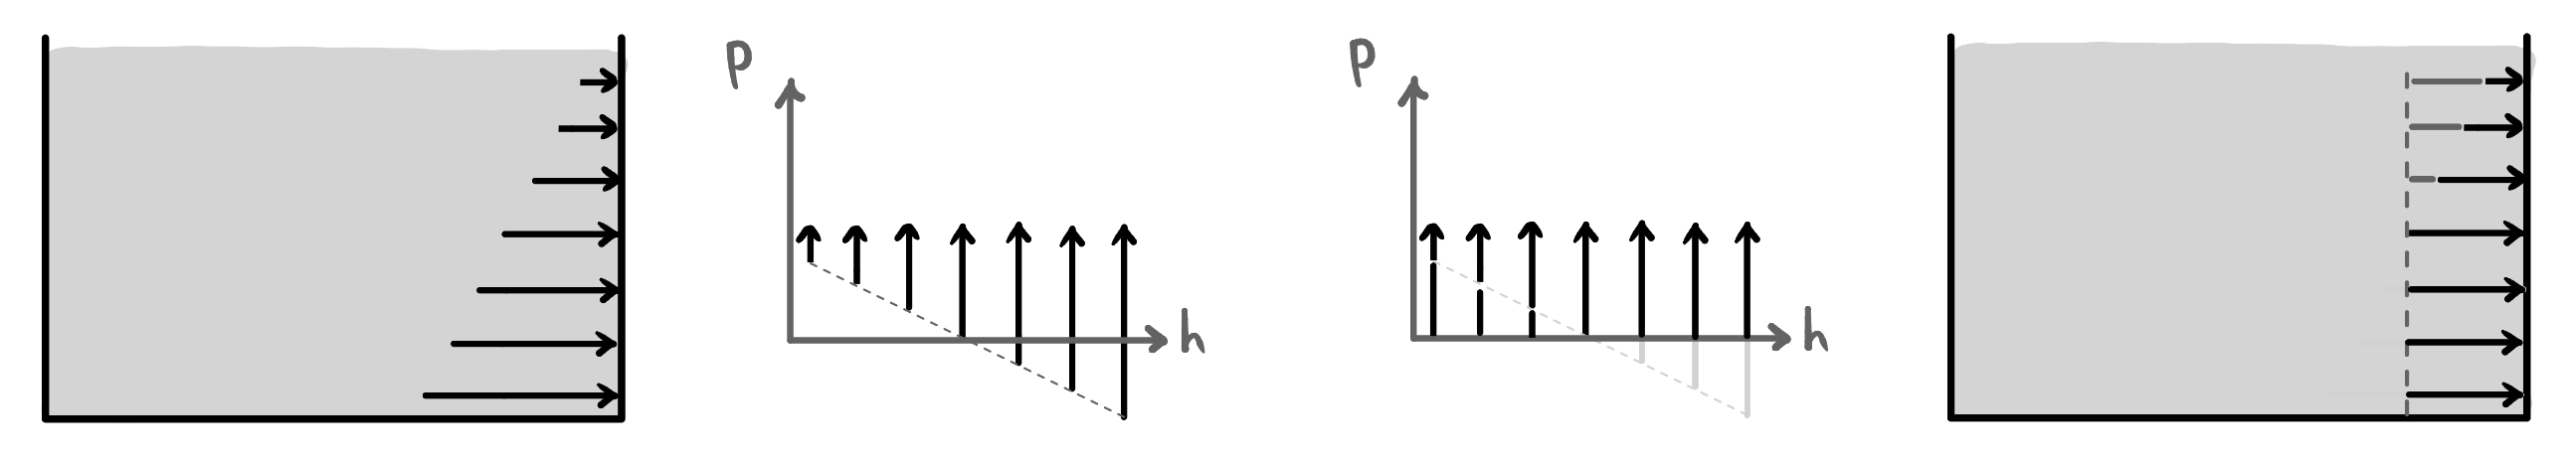
\includegraphics[width=0.95\linewidth]{imagensfluidos/pressaoforcamedia.png}};
  \end{scope}
\end{tikzpicture}
\captionof{figure}{}
\label{fig_fluidos_pressaoforcamedia}
} 
\vspace{0.3cm}

Como a função varia de forma linear em $y$, pontos equidistantes de um ponto médio $M$ possuem variações que se compensam: um ponto $P$ que está 10 cm acima do ponto médio $M$ possui menos pressão do que o ponto $M;$ porém um ponto $Q$ que está 10 cm abaixo do ponto médio $M$ possui mais pressão do que o ponto $M,$ e exatamente o mesmo tanto a mais (por ser linear) do que o ponto $P$ possui de pressão a menos. Assim, essas variações se compensam e a pressão gerada por $P$ e $Q,$ juntos, fica sendo exatamente igual à pressão do seu ponto médio $M$.

Desse modo, para computar a força total que a água exerce na parede lateral da barreira, podemos considerar, como mostra a última imagem da Figura \ref{fig_fluidos_pressaoforcamedia}, que a pressão em toda a parede lateral é constante, e igual à pressão do seu ponto médio. Assim, aplicando $F=P_M \cdot A,$ em que $P_M$ é a pressão do ponto médio, obtém-se o resultado exato da força exercida pela água em tal parede.
 

 \medskip

 
\textit{c)} Analisando os casos limites de \eqref{eq:F_estimativa}:
 
\textbf{Caso $P_0 \to 0$ (superfície sob vácuo):}
 
\begin{equation*}
    F\big|_{P_0 = 0} = \frac{\rho g H^2}{2}\,L
\end{equation*}
 
Resta apenas a contribuição do peso do fluido. Fisicamente: se não
há pressão atmosférica pressionando a superfície, a única origem de
pressão sobre a parede é a própria coluna de água acima de cada ponto.
Na base, essa pressão é $\rho g H$; na superfície, é zero. A força
resultante é a área do triângulo formado pelo perfil de pressão:
base $\rho g H$, altura $H$, área $\rho g H^2 / 2$~--- multiplicada
por $L$.
 
\textbf{Caso $\rho \to 0$ (fluido sem peso):}
 
\begin{equation*}
    F\big|_{\rho = 0} = P_0\,H\,L
\end{equation*}
 
A pressão sobre a parede é uniforme e igual a $P_0$ em todos os
pontos. A força é simplesmente pressão vezes área~--- o caso mais
elementar de $\mathcal{P} = F/A$. 

\medskip
 
\textit{d)} As duas parcelas de \eqref{eq:F_estimativa} são:
 
\begin{equation*}
    F_{P_0} = P_0\,H\,L
    \qquad \text{e} \qquad
    F_{\rho} = \frac{\rho g H^2}{2}\,L
\end{equation*}
 
A razão entre elas:
 
\begin{equation}
    \frac{F_{\rho}}{F_{P_0}}
    = \frac{\rho g H^2 / 2}{P_0 H}
    = \frac{\rho g H}{2 P_0}
    \label{eq:razao_parcelas}
\end{equation}
 
As parcelas se igualam quando $F_{\rho}/F_{P_0} = 1$:
 
\begin{equation}
    \frac{\rho g H^*}{2 P_0} = 1
    \implies
    \boxed{H^* = \frac{2 P_0}{\rho g}}
    \label{eq:H_estrela}
\end{equation}
 
Para água ($\rho = \SI{e3}{\kilo\gram\per\metre\cubed}$) e
$P_0 = \SI{e5}{\pascal}$:
 
\begin{equation*}
    H^* = \frac{2 \cdot 10^5}{10^3 \cdot 10} = \SI{20}{\metre}
\end{equation*}
 
Para barragens com $H < \SI{20}{\metre}$, a pressão atmosférica domina
a força sobre a parede. Para $H > \SI{20}{\metre}$, o peso do fluido
passa a dominar~--- e como $F_\rho \propto H^2$, esse domínio cresce
rapidamente com a altura. É por essa razão que grandes barragens
exigem fundações e estruturas de contenção radicalmente mais robustas
do que barragens de menor porte: a força cresce quadraticamente, não
linearmente, com a altura da coluna de água.

\end{exemplo}

\vspace{0.3cm}








\begin{secnivel}[Empuxo]{I}{Empuxo}
  
  \eqLdois{dem}{eq_fluidos_empuxo}{E = \rho V_{\text{D}}g}

\end{secnivel}







\secgfe{De onde vem}

Antes de qualquer equação, vamos a uma bela história. Arquimedes de Siracusa, matemático e filósofo do século III a.C., recebeu do rei Hierão II uma missão delicada: verificar se a coroa real era de ouro puro ou se o ourives havia misturado prata na liga. O problema era claro — a coroa tinha a massa certa —, mas seria ela integralmente feita de ouro? Segundo a lenda, a resposta veio na banheira. Ao entrar na água, Arquimedes percebeu que seu corpo deslocava um volume de água e que o fluido, de alguma forma, ``empurrava'' para cima. Correu pelas ruas nu, gritando \textit{Eureka!} A física que ele intuiu naquele momento, porém, exige que a matematizemos com cuidado.
 
Para entender de onde vem o empuxo, o leitor precisa ter bem firme o que aprendemos na seção sobre a Equação \eqref{eq_fluidos_leidestevin}: a pressão em um fluido em equilíbrio cresce com a profundidade. É exatamente essa variação de pressão que vai originar a força de empuxo.

Considere a Figura \ref{fig_fluidos_empuxo01}. A primeira imagem mostra, em linha pontilhada, uma certa porção de líquido que vamos analisar. Todo o líquido do aquário está em equilíbrio, e possui densidade $\rho.$


\vspace{0.3cm}
{
\centering
\begin{tikzpicture}
  \begin{scope}[blend mode=multiply]
    \node {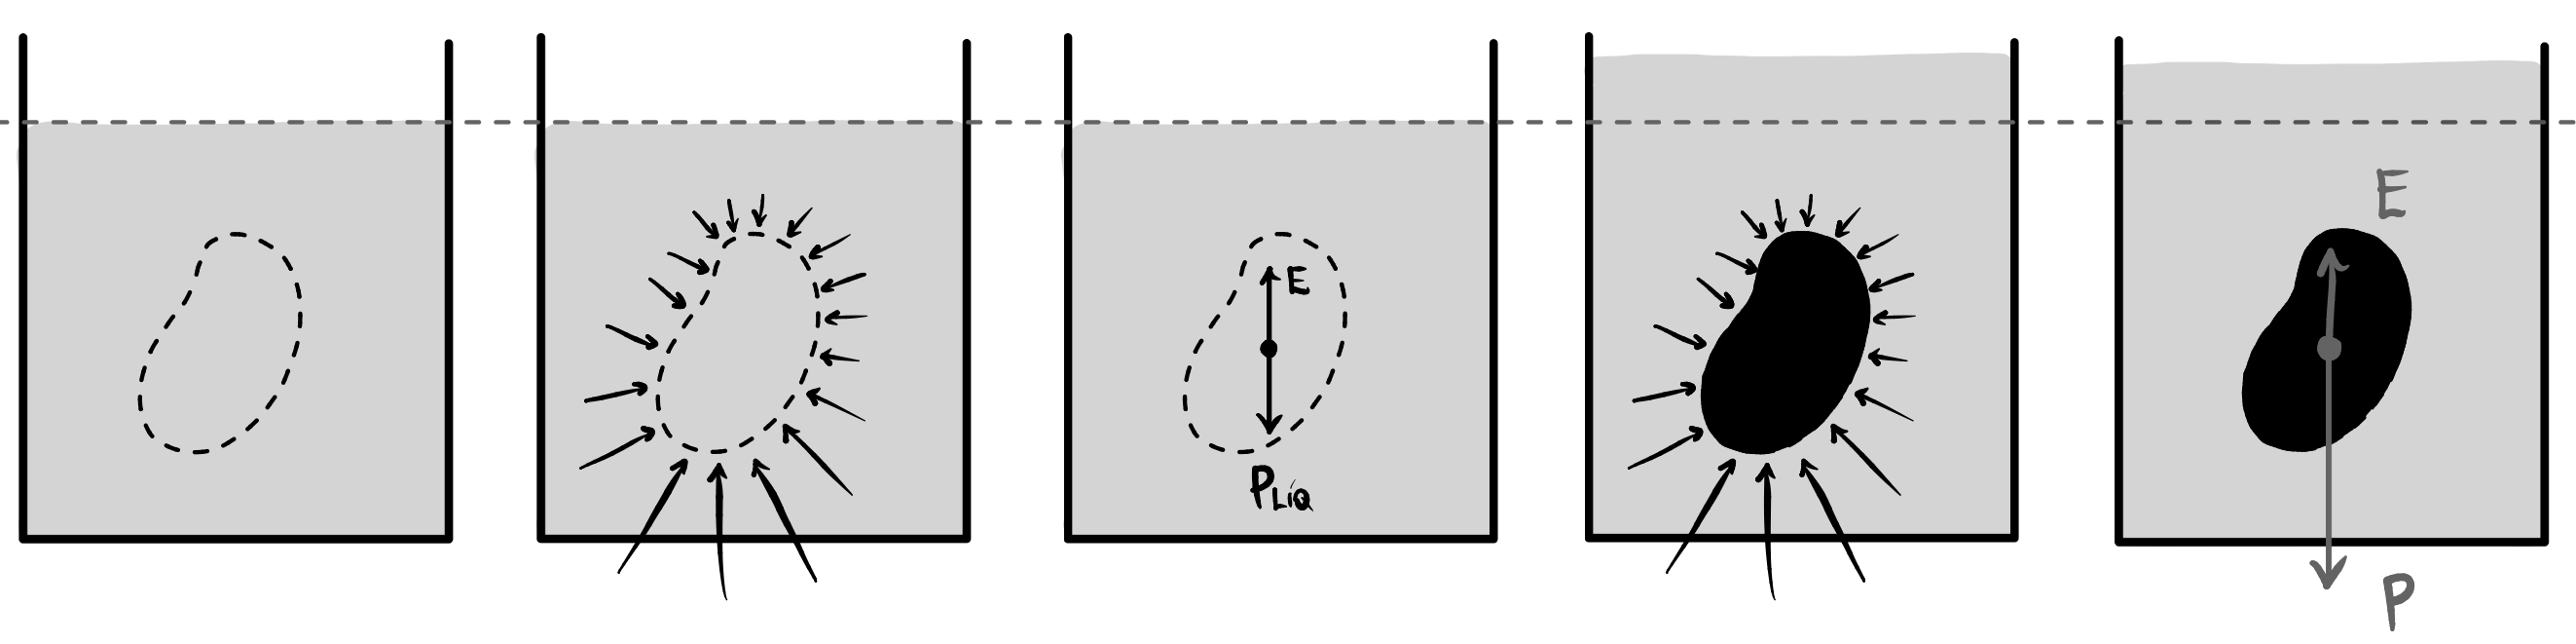
\includegraphics[width=0.95\linewidth]{imagensfluidos/empuxodemonstracao1.png}};
  \end{scope}
\end{tikzpicture}
\captionof{figure}{Um corpo imerso em um fluido sente uma força verticalmente para cima igual ao peso do fluido deslocado por ele.}
\label{fig_fluidos_empuxo01}
} 
\vspace{0.3cm}


A segunda imagem mostra a distribuição de pressão ao longo dessa porção de líquido: quanto maior a profundidade, maior é a pressão. Isso faz com que a pressão embaixo seja maior do que a pressão em cima, gerando uma diferença de pressão responsável por gerar uma força de sustentação $E,$ verticalmente para cima, como mostra a terceira imagem da figura. No caso, como a porção de líquido em questão está em equilíbrio -- lembre-se, estamos em situação de hidrostática -- a força resultante deve ser nula, de tal modo que o empuxo deve ser exatamente igual ao seu peso:

$$ E = P_\text{LIQ} \implies E = m_\text{LIQ}g.$$

E, sendo $\rho = m/V,$ podemos escrever que

\begin{equation}
     E = \rho V_\text{LIQ}g, 
     \label{eq_fluido_manipulacaoempuxo}
\end{equation}

\noindent em que $V$ é o volume da porção de líquido em questão. 


Agora, note que, ao inserir um objeto -- digamos, uma pedra -- que possui exatamente o mesmo formato geométrico e ocupa exatamente o mesmo volume da tal porção de líquido analisada, duas coisas importantes ocorrem:

\begin{enumerate}
    \item [(i)] O nível da água no recipiente sobe. Isso ocorre porque a região do espaço antes ocupada pelo fluido agora é ocupada pela pedra. Desse modo, ao inserir um objeto em um fluido, tal objeto \emph{desloca} um volume de fluido exatamente igual ao seu próprio volume que foi submerso, haja vista que dois corpos não podem ocupar o mesmo lugar do espaço simultaneamente.

    É isso que permitiu que Arquimedes compreendesse o material da coroa do rei: materiais de diferentes densidades (prata e ouro, no caso) irão ocupar volumes diferentes para uma mesma massa, de modo que deslocarão quantidades diferentes de fluidos ao serem imersos.


    \item [(ii)] Tendo a pedra exatamente o mesmo volume e formato geométrico da porção de fluido analisada, é fácil notar que a distribuição de pressão externa fica inalterada. Ou seja, a distribuição de pressão da segunda imagem da Figura \ref{fig_fluidos_empuxo01} se mantém quando a pedra é inserida, haja vista que o fluido ``não sabe'' se o que tem naquele volume do espaço é uma pedra ou o próprio fluido -- a distribuição de pressões é algo externo a tal volume, que depende do líquido em seu entorno, e não do corpo em si que ocupa aquele volume. A quarta imagem da figura destaca isso.

    Sendo assim, a pedra sentirá uma força de sustentação vertical, para cima, cujo módulo é exatamente igual ao peso da quantidade de líquido deslocado por ela. A tal força damos o nome de empuxo, e isso está representado na última imagem da Figura \ref{fig_fluidos_empuxo01}.\footnote{Na última imagem note que $P$ é o peso da pedra, o qual não precisa ser igual ao empuxo $E.$ Caso ele seja, a pedra ficaria flutuando, em equilíbrio, em tal posição. Se o peso da pedra for maior, ela afundaria a partir de tal posição e, caso fosse menor, ela subiria e ficaria em equilíbrio na superfície do fluido, com parte do seu volume submerso. Veremos, em breve, que esses fatos estão relacionados com a densidade da pedra em relação à densidade do fluido.}
    
    
    Como visto, ele é exatamente igual ao peso da quantidade de fluido \textbf{deslocado} por um objeto imerso na água. Desse modo, para que não se confunda o volume do corpo imerso com o volume do líquido que foi deslocado, colocamos o subíndice $D$ no volume $V$ na Equação \eqref{eq_fluido_manipulacaoempuxo}, de modo que somos levados exatamente à Equação \eqref{eq_fluidos_empuxo}: $E= \rho V_D g,$ em que $\rho$ é a densidade do fluido, $V_D$ é o volume de fluido deslocado e $g$ é a aceleração da gravidade.

    Esse detalhe do volume deslocado é muito importante, haja vista que um mesmo corpo, a depender de como ele está imerso no fluido, poderá sentir diferentes empuxos. A Figura \ref{fig_fluidos_empuxo02} mostra isso: tem-se a mesma bola, nas três situações, porém em cada uma delas a quantidade do seu volume imersa é diferente. Em cada situação, portanto, o empuxo terá um valor diferente. O valor numérico $V_D$ a ser inserido na \eqref{eq_fluidos_empuxo} será igual ao volume da bola que está dentro d'água, que se encontra hachurado nas figuras. O empuxo será mínimo na primeira situação e máximo na última.

\vspace{0.3cm}
{
\centering
\begin{tikzpicture}
  \begin{scope}[blend mode=multiply]
    \node {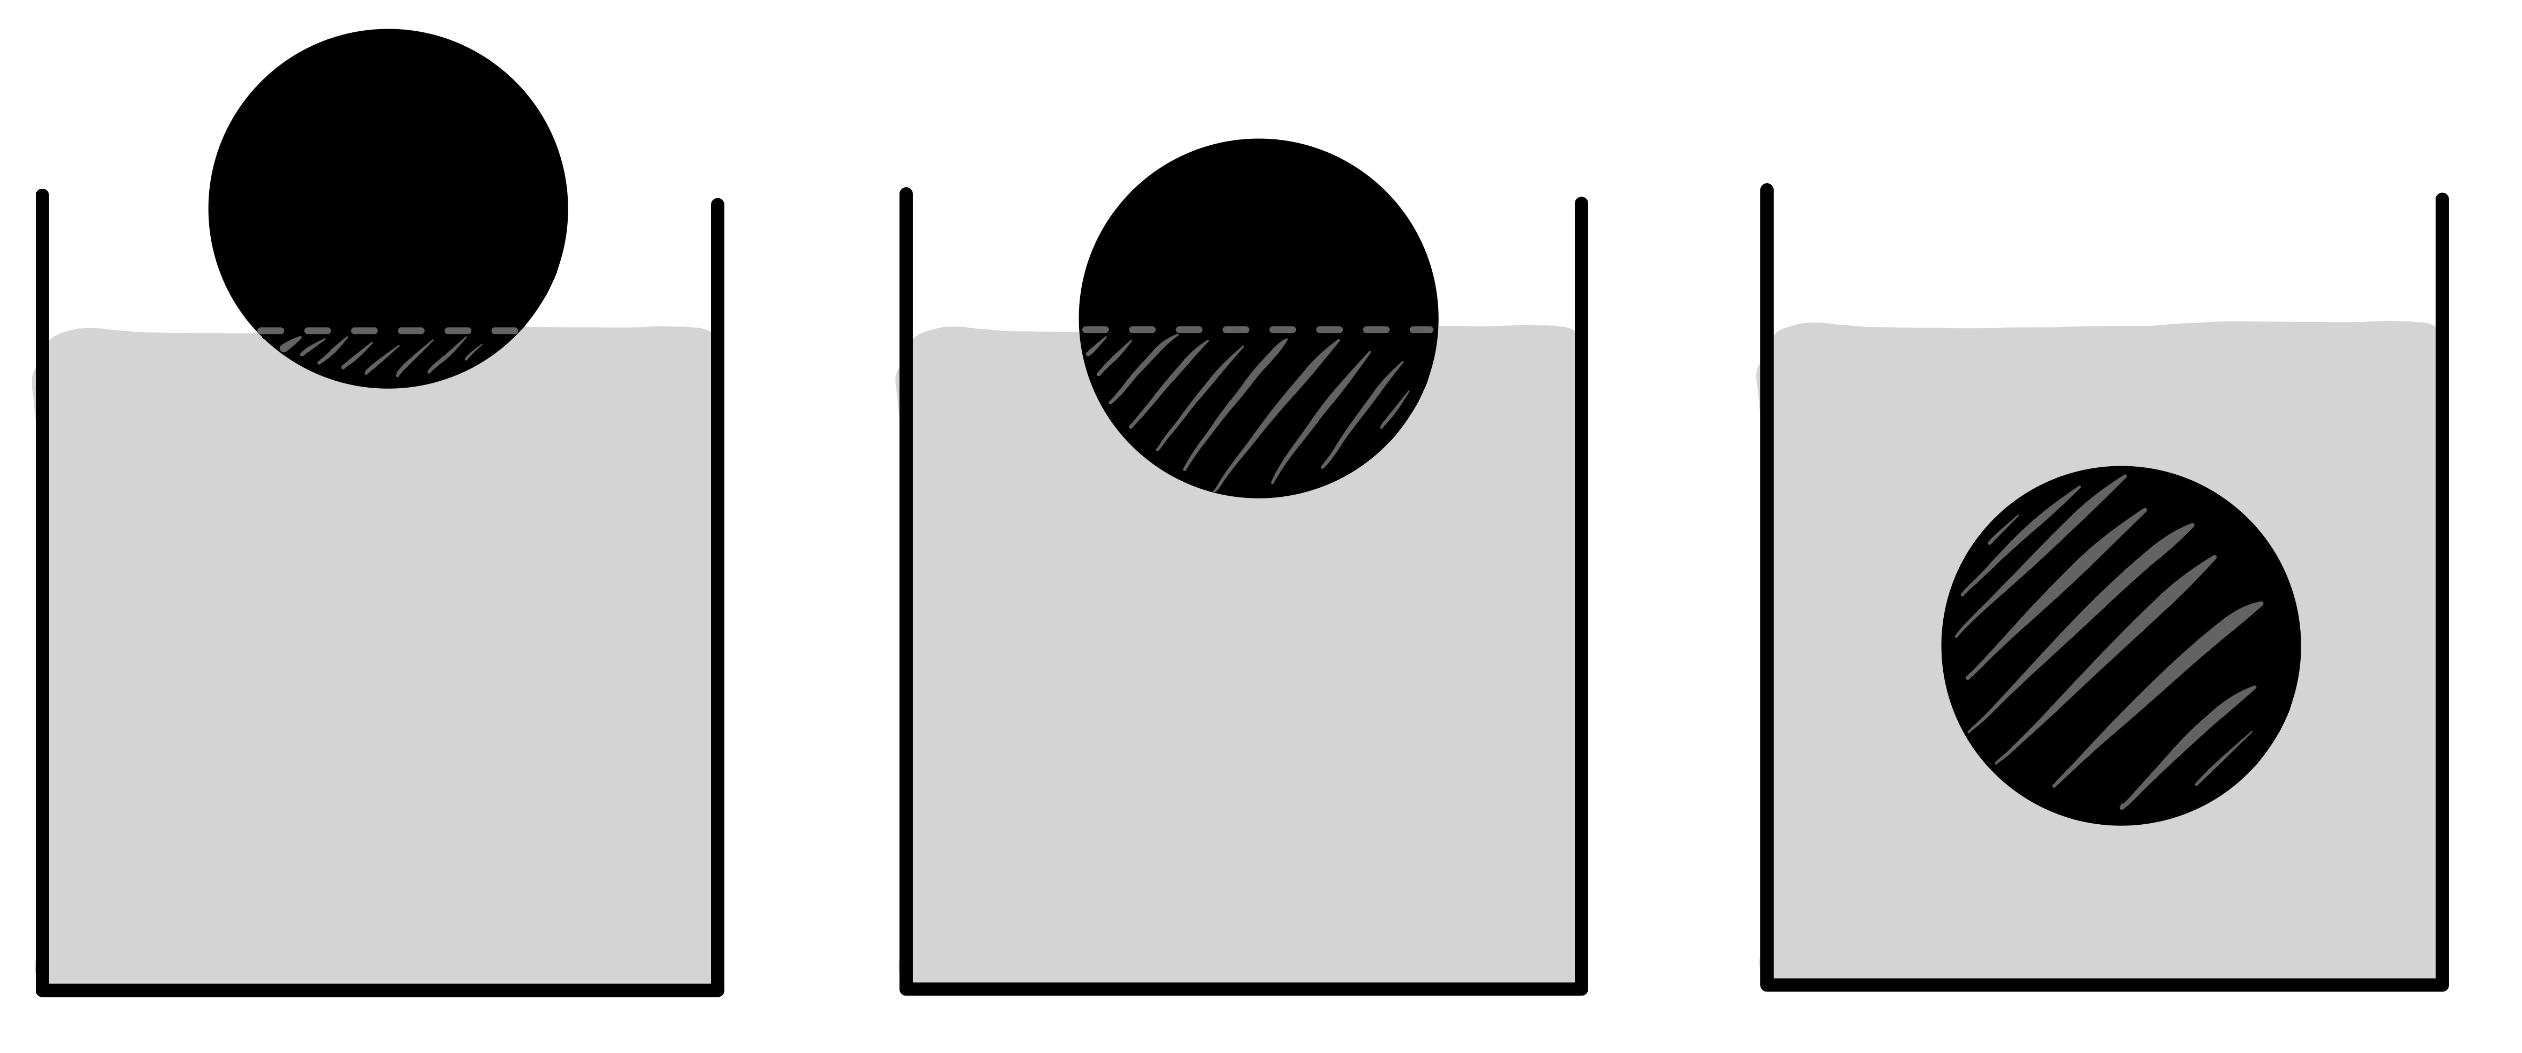
\includegraphics[width=0.5\linewidth]{imagensfluidos/empuxodemonstracao3.png}};
  \end{scope}
\end{tikzpicture}
\captionof{figure}{O empuxo está relacionado ao volume submerso do corpo: ele é exatamente igual ao peso do líquido que ocupava tal volume.}
\label{fig_fluidos_empuxo02}
} 
\vspace{0.3cm}


\end{enumerate}


É por isso que temos a sensação de que os objetos ficam mais leves dentro d'água: você não precisa sustentar todo o seu peso, haja vista que o empuxo já faz uma parcela dessa força. Como mostra a última imagem da Figura \ref{fig_fluidos_empuxo01}, a força vertical $F$ necessária para manter em equilíbrio o objeto é tal que 

$$ F_\text{R} = 0 \implies E + F = P \implies F = P - E.$$


A isso damos o nome de \emph{peso aparente:} a diferença entre o peso real do objeto e o empuxo que ele sente. Essa é exatamente a força extra que alguém teria que fazer para sustentar tal objeto, de modo que tem-se a impressão de que ele é mais leve. Considere um objeto de massa $m=$1kg, de modo que seu peso é $P=10$ N. Assuma que ele está imerso em um fluido de tal modo que $E=4$ N. Você precisa fazer apenas $(10-4)=6$ N de força vertical para cima para sustentar tal objeto, o que equivale ao peso de um objeto de $600$g, e não de $1$kg, como de fato é o caso. Sua impressão é que o objeto ficou mais leve -- este é o conceito de \emph{peso aparente.}

\secgfe{Onde é usada}


O empuxo é extremamente importante para garantir que corpos imersos em um fluido estejam em equilíbrio. Um navio, por exemplo, possui um alto volume que deve ficar submerso -- chamado de calado -- de tal modo que o empuxo consiga equilibrar o peso do navio. Assim, é preciso aplicar a Equação \eqref{eq_fluidos_empuxo} para descobrir qual é o exato volume $V_D$ do calado a fim de gerar um empuxo que consiga equilibrar o peso do navio para que ele não afunde.

\vspace{0.3cm}
{
\centering
\begin{tikzpicture}
  \begin{scope}[blend mode=multiply]
    \node {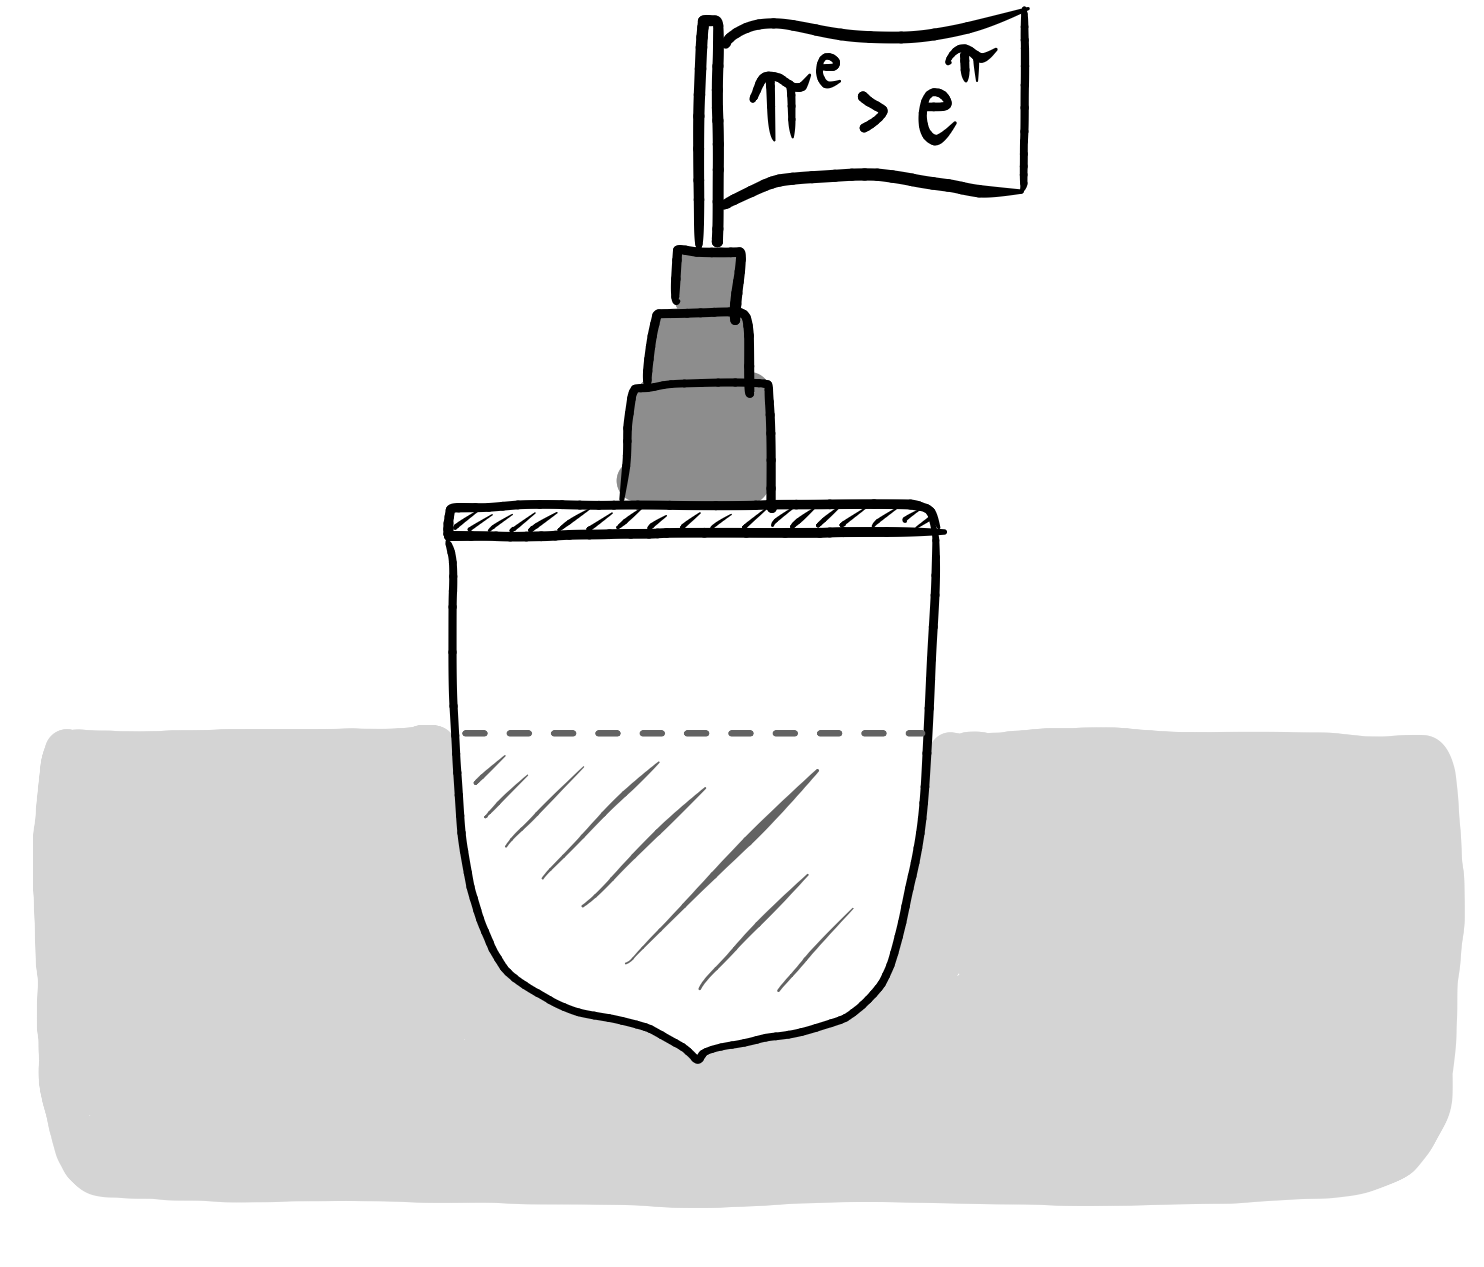
\includegraphics[width=0.35\linewidth]{imagensfluidos/empuxonavio.png}};
  \end{scope}
\end{tikzpicture}
\captionof{figure}{O calado é a região do navio que fica imersa dentro d'água.}
\label{fig_fluidos_empuxonavio}
} 
\vspace{0.3cm}

Ainda nesse contexto, é a densidade relativa de um corpo em relação à densidade do fluido que determina se ele irá afundar ou flutuar em tal fluido, abandonado em repouso naquela posição. Considere, por exemplo, a situação da terceira imagem da Figura \ref{fig_fluidos_empuxo02}, em que temos um corpo totalmente submerso em um certo fluido. Temos, a partir de tal configuração, três situações possíveis:

\begin{enumerate}
    \item [(i)] O corpo afunda.

    Para isso, é necessário que seu peso seja maior que o empuxo, ou seja: 

    $$ P > E \implies m \cancel g > \rho_{LIQ} V \cancel g  \implies \rho \cancel V > \rho_{LIQ} \cancel V  \implies \boxed{\rho > \rho_{LIQ},}$$

    \noindent ou seja, o corpo irá afundar caso ele seja mais denso do que o líquido. Nesse desenvolvimento usamos que $\rho$ é a densidade do corpo, e, de $\rho = m/V,$ escrevemos que $m= \rho V.$ Note que, como o corpo está totalmente submerso, o volume de líquido deslocado é igual ao seu volume, isto é, $V_D = V.$

      \item [(ii)] O corpo fica em equilíbrio nessa posição.

    Para isso, é necessário que seu peso seja exatamente igual ao empuxo, ou seja: 

    $$ P = E \implies m \cancel g = \rho_{LIQ} V \cancel g  \implies \rho \cancel V = \rho_{LIQ} \cancel V  \implies \boxed{\rho = \rho_{LIQ},}$$

    \noindent ou seja, o corpo irá ficar em equilíbrio totalmente imerso no fluido, flutuando exatamente naquela posição, caso ele tenha exatamente a mesma densidade que o líquido.


        \item [(iii)] O corpo irá acelerar para cima, subindo ao longo do fluido.

    Para isso, é necessário que seu peso seja menor que o empuxo, ou seja: 

    $$ P < E \implies m \cancel g < \rho_{LIQ} V \cancel g  \implies \rho \cancel V < \rho_{LIQ} \cancel V  \implies \boxed{\rho < \rho_{LIQ},}$$

    \noindent ou seja, o corpo precisa ser menos denso que o fluido. Neste caso ele iria acelerar para cima, ficando em equilíbrio com seu volume parcialmente imerso no fluido, como na situação da primeira imagem da Figura \ref{fig_fluidos_empuxo02}, por exemplo.
\end{enumerate}









\secgfe{Erros comuns}

Um erro bastante comum é confundir uma consequência da Equação \eqref{eq_fluidos_leidestevin} e aplicar ela no empuxo. Considere, por exemplo, a situação da primeira imagem da Figura \ref{fig_fluidos_empuxo03}, que mostra duas pedras idênticas totalmente imersas em um certo fluido. Em qual das duas o empuxo é maior?

\vspace{0.3cm}
{
\centering
\begin{tikzpicture}
  \begin{scope}[blend mode=multiply]
    \node {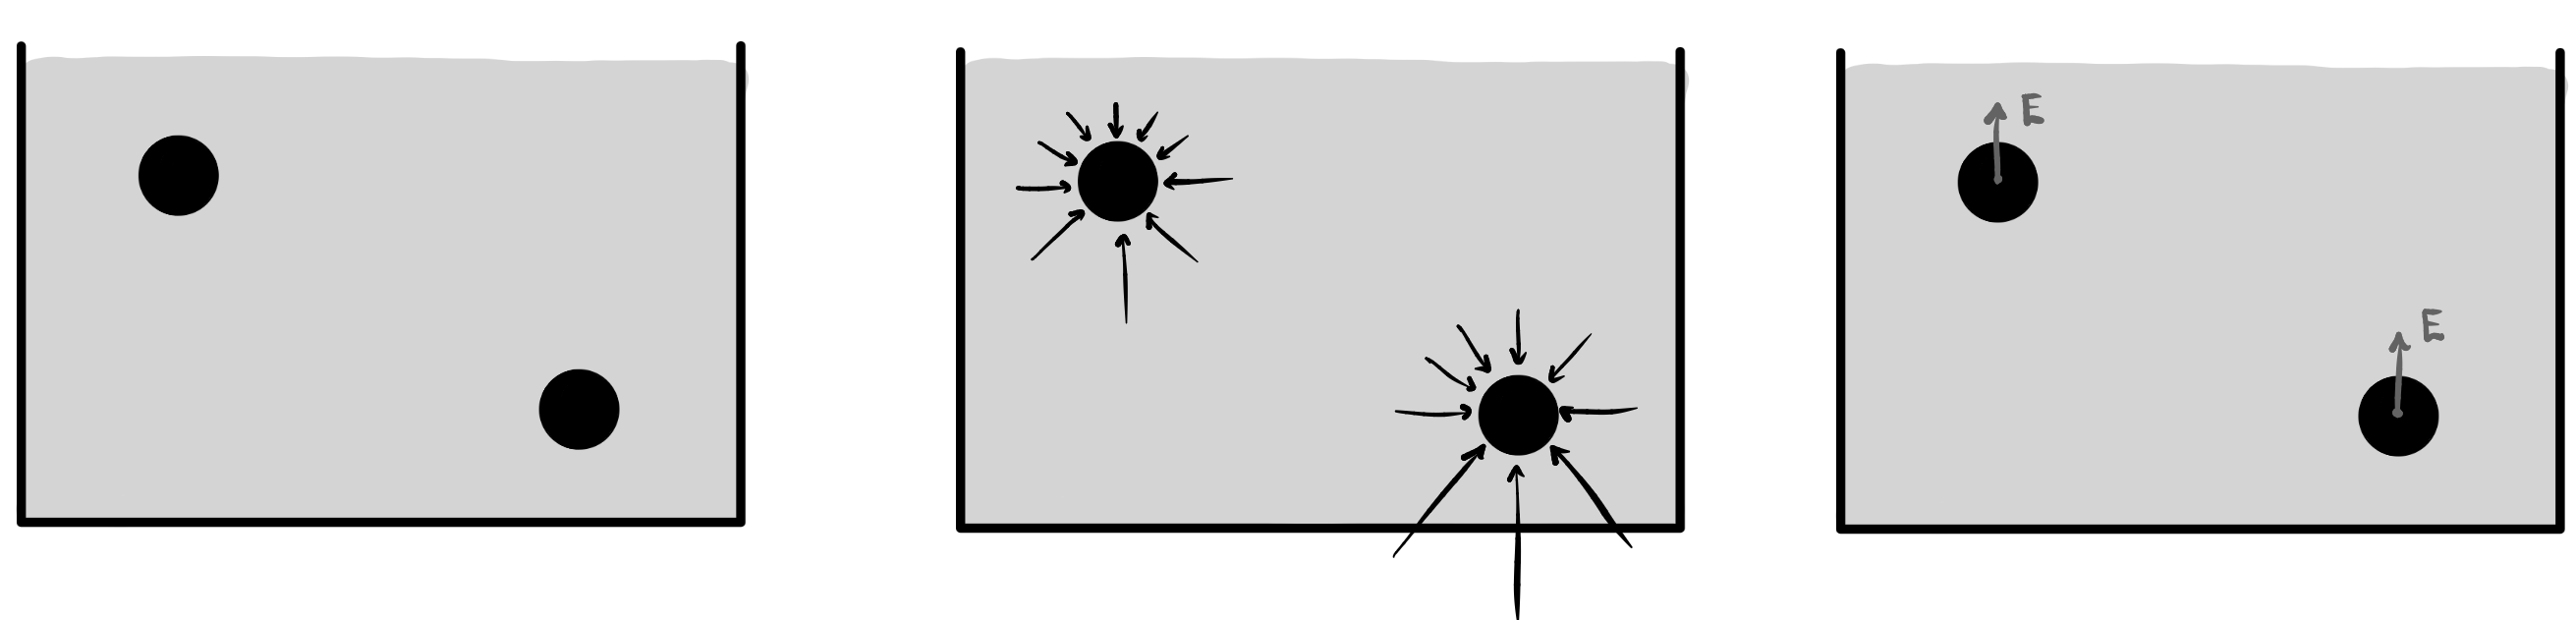
\includegraphics[width=0.8\linewidth]{imagensfluidos/empuxodemonstracao2.png}};
  \end{scope}
\end{tikzpicture}
\captionof{figure}{O empuxo não depende da profundidade.}
\label{fig_fluidos_empuxo03}
} 
\vspace{0.3cm}

O leitor poderia pensar que o empuxo seria maior na pedra da direita, que está mais no fundo, haja vista que a pressão é maior quanto maior for a profundidade, como diz a Equação \eqref{eq_fluidos_leidestevin}. Este último fato até está correto, já a conclusão de que isso implica no empuxo sob a pedra da direita ser maior é equivocada. Isso porque o empuxo está relacionado, como mostra a segunda imagem da Figura \ref{fig_fluidos_empuxo01}, à \textit{diferença de pressão}, e não à pressão em si. Desse modo, a pressão na pedra que está mais no fundo de fato é maior: mas ela é maior tanto em cima dela, empurrando-a para baixo; quanto em baixo, empurrando-a para cima. Isso aparece na segunda imagem da Figura \ref{fig_fluidos_empuxo03}.

Desse modo, a diferença de pressão acaba sendo a mesma, haja vista que ela depende apenas da altura $\Delta h$ da pedra, dada por $\Delta p = \rho g \Delta h,$ como sabemos. Assim, as duas pedras sentirão exatamente o mesmo empuxo, como mostra a terceira imagem da figura. O empuxo, portanto, não depende da profundidade. Como a própria equação \eqref{eq_fluidos_empuxo} destaca, do ponto de vista do objeto que foi inserido no fluido, o empuxo depende exclusivamente do volume de líquido deslocado $V_D$, não dependendo do formato geométrico específico do corpo ou de qual é a profundidade na qual ele se encontra.





\secgfe{Observações}

Até então, tudo o que falamos -- sobre a definição de empuxo e como calculá-lo -- está relacionado ao que chamamos de \emph{empuxo arquimediano.} Considere, contudo, a situação da Figura \ref{fig_fluidos_empuxonaoarquimediano}, que mostra uma caixa cúbica, de aresta $a$, mais densa do que o fluido e que, portanto, afundou, ficando em equilíbrio no fundo do aquário. Veremos que o cálculo -- e o próprio conceito -- do empuxo será diferente nessa situação.


\vspace{0.3cm}
{
\centering
\begin{tikzpicture}
  \begin{scope}[blend mode=multiply]
    \node {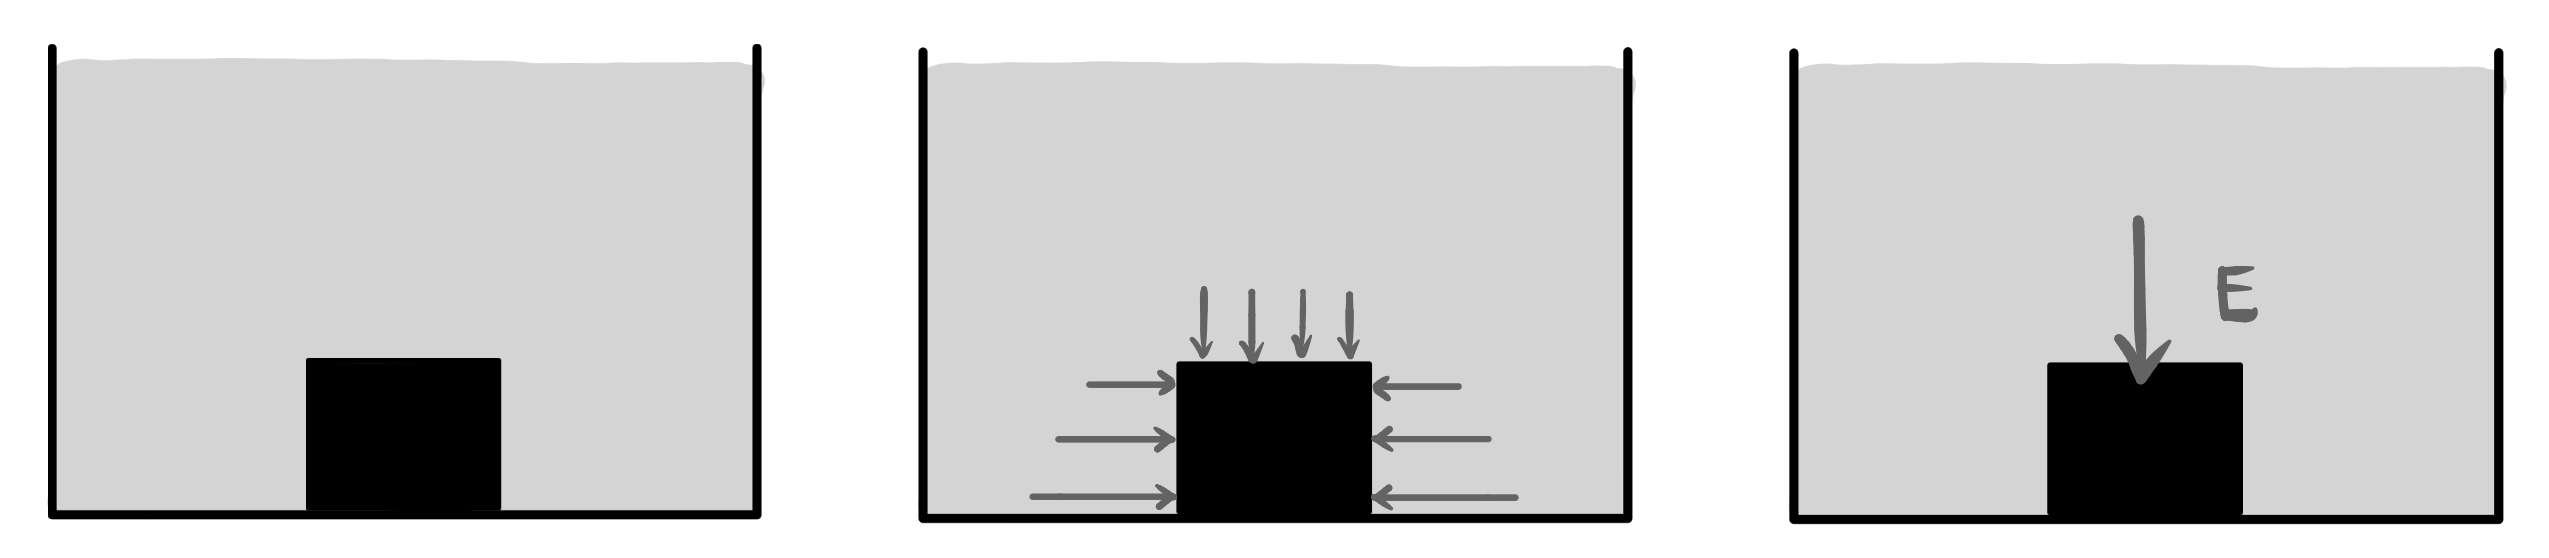
\includegraphics[width=0.75\linewidth]{imagensfluidos/empuxonaoaruimediano.png}};
  \end{scope}
\end{tikzpicture}
\captionof{figure}{O empuxo não arquimediano.}
\label{fig_fluidos_empuxonaoarquimediano}
} 
\vspace{0.3cm}

Avaliemos como são as pressões que o bloco sente: ele é comprimido para baixo devido à pressão do peso da coluna de fluido acima dele. Além disso, ele sente pressões nas suas laterais -- efeitos que se anulam, por simetria. Note, contudo, que por estar pregado no fundo do aquário, não existe a pressão do fluido embaixo do bloco, empurrando ele para cima, e responsável por gerar o empuxo conforme havíamos estudado.

Nessa situação, portanto, o empuxo, como mostra a terceira imagem da figura, será vertical para baixo: é a força do peso da coluna de fluido acima da caixa. Chamamos esse empuxo de \emph{não arquimediano.} 

Neste caso, sendo $h$ a altura da coluna de fluido acima do bloco, ela teria um volume total $V = a^2h$, em que $a$ é a aresta do cubo, e um peso $P = mg = \rho V g = \rho a^2hg.$ Assim, o empuxo sentido pela caixa seria uma força de compressão vertical e para baixo, cujo módulo é $E = \rho a^2hg, $ em que $\rho$ é a densidade do fluido.





\vspace{0.3cm}


\begin{exemplo}[Nível I]\label{exemplo_fluidos_empuxoex01}

Uma peça de madeira tem volume $500\text{ cm}^3$ e massa $400\text{ g}$. Ela é colocada sobre água parada. A peça flutua ou afunda? Se flutuar, qual fração do volume fica submersa?

\resolucao

Antes de qualquer conta, calculemos a densidade da madeira:
 
\begin{equation*}
    \rho_\text{mad} = \frac{m}{V} = \frac{0{,}4}{5\cdot 10^{-4}} = 800\ \text{kg/m}^3.
\end{equation*}
 
Como $\rho_\text{mad} = 800\ \text{kg/m}^3 < \rho_\text{água} = 1\,000\ \text{kg/m}^3$, a peça \textit{flutua}. Para encontrar a fração submersa, impomos o equilíbrio entre empuxo e peso:
 
\begin{equation*}
    E = P \implies \rho_\text{água} \cdot V_\text{sub} \cdot g = m \cdot g
\end{equation*}
 
\begin{equation*}
    V_\text{sub} = \frac{m}{\rho_\text{água}} = \frac{0{,}4}{1\,000} = 4 \cdot 10^{-4}\ \text{m}^3
\end{equation*}
 
A fração submersa é:
 
\begin{equation*}
    \frac{V_\text{sub}}{V_\text{obj}} = \frac{4\cdot10^{-4}}{5\cdot10^{-4}} = \frac{4}{5} = \boxed{80\%.}
\end{equation*}
 
Oitenta por cento da madeira ficam abaixo da linha d'água. Poderíamos ter chegado ao mesmo resultado pela razão entre as densidades $\rho_\text{obj}/\rho_\text{liq} = 800/1\,000 = 0{,}8$.

\end{exemplo}




\vspace{0.3cm}


\begin{exemplo}[Nível II]\label{exemplo_fluidos_empuxoex02}

Uma coroa suspeita tem massa $m = 500\ \text{g}$. Pendurada por um fio dentro de água, a balança de mola registra um peso aparente de $4{,}55\ \text{N}$. Sabendo que $\rho_\text{ouro} = 19\,300\ \text{kg/m}^3$ e $\rho_\text{prata} = 10\,500\ \text{kg/m}^3$, determine a densidade da coroa e avalie se ela é de ouro puro.
 
 
\medskip

\resolucao

O peso real da coroa no ar é $P_\text{ar} = mg = 5\ \text{N}$. Quando a coroa é submersa, a balança deixa de medir seu peso real e passa a medir o chamado \textit{peso aparente}: a resultante do peso real para baixo e do empuxo para cima. O empuxo é, portanto, a diferença entre os dois registros:
 
\begin{equation*}
    E = P_\text{ar} - P_\text{ap} = 5{,}00 - 4{,}55 = 0{,}45\ \text{N}
\end{equation*}
 
Com o valor do empuxo, extraímos o volume da coroa:
 
\begin{equation*}
    E = \rho_\text{água}\cdot V\cdot g
    \implies
    V = \frac{E}{\rho_\text{água}\cdot g} = \frac{0{,}45}{1\,000\cdot 10} = 4{,}5\cdot10^{-5}\ \text{m}^3
\end{equation*}
 
A densidade da coroa é, então:
 
\begin{equation*}
    \rho_\text{coroa} = \frac{m}{V} = \frac{0{,}5}{4{,}5\cdot10^{-5}} \approx \boxed{11.111\ \text{kg/m}^3}
\end{equation*}
 
A coroa \textbf{não} é de ouro puro ($\rho_\text{ouro} = 19\,300\ \text{kg/m}^3$). Sua densidade está entre a do ouro e a da prata — exatamente o resultado que Arquimedes apresentou ao rei Hierão: uma liga adulterada com prata ocupa mais volume por quilograma e, por isso, desloca mais água do que deslocaria se fosse ouro maciço. O método é elegante justamente por ser bastante simples.

\end{exemplo}




\vspace{0.3cm}


\begin{exemplo}[Nível III (ITA - 2014)]\label{exemplo_fluidos_empuxoex03}

Uma esfera de massa $m$ tampa um buraco circular de raio $r$ no fundo de um recipiente cheio de água de massa específica $\rho$. Baixando-se lentamente o nível da água, num dado momento a esfera se desprende do fundo do recipiente. Assinale a alternativa que expressa a altura $h$ do nível de água para que isto aconteça, sabendo que o topo da esfera, a uma altura $a$ do fundo do recipiente, permanece sempre coberto de água.

\vspace{0.5cm}

\begin{center}
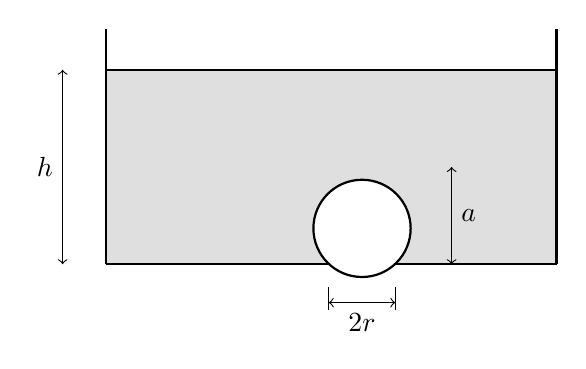
\begin{tikzpicture}[scale=0.65]

 % dimensões principais
    \def\H{4.6}         % altura do recipiente
    \def\W{8.8}         % largura do recipiente
    \def\hwater{3.8}    % nível da água

    % esfera
    \def\R{0.95}
    \def\cx{5.0}
    \def\cy{0.70}       % tangente ao fundo y=0

    % furo
    \def\holeL{4.35}
    \def\holeR{5.65}

    % paredes do recipiente
    \draw[thick] (0,0) -- (0,\H);
    \draw[thick] (\W,0) -- (\W,\H);

    % fundo com abertura
    \draw[thick] (0,0) -- (\holeL,0);
    \draw[thick] (\holeR,0) -- (\W,0);

    % região da água
    \fill[gray!25] (0,0) rectangle (\W,\hwater);

    % "recorte" da esfera para ela aparecer sobre a água
    \fill[white] (\cx,\cy) circle (\R);
    \draw[thick] (\cx,\cy) circle (\R);

    % redesenha partes visíveis do recipiente
    \draw[thick] (0,\hwater) -- (\W,\hwater);
    \draw[thick] (0,0) -- (\holeL,0);
    \draw[thick] (\holeR,0) -- (\W,0);
    \draw[thick] (0,0) -- (0,\H);
    \draw[thick] (\W,0) -- (\W,\H);

    % cota h
    \draw[<->] (-0.85,0) -- (-0.85,\hwater);
    \node[left] at (-0.85,0.5*\hwater) {$h$};

    % cota a
    \draw[<->] (\cx+\R+0.8,0) -- (\cx+\R+0.8,2*\R);
    \node[right] at (\cx+\R+0.8,\R) {$a$};

    % cota 2r
    \draw (\holeL,-0.45) -- (\holeL,-0.9);
    \draw (\holeR,-0.45) -- (\holeR,-0.9);
    \draw[<->] (\holeL,-0.75) -- (\holeR,-0.75);
    \node[below] at ({(\holeL+\holeR)/2},-0.78) {$2r$};

\end{tikzpicture}
\end{center}


\vspace{0.5cm}

\begin{enumerate}
    \item [a)] $ \dfrac{m}{\rho\pi a^2}$
    \item [b)] $ \dfrac{m}{\rho\pi r^2}$
    \item [c)] $ \dfrac{a(3r^2+a^2)}{6r^2}$
    \item [d)] $ \dfrac{a}{2}-\dfrac{m}{\rho\pi r^2}$
    \item [e)] $ \dfrac{a(3r^2+a^2)}{6r^2}-\dfrac{m}{\rho\pi r^2}$
\end{enumerate}


\resolucao


A primeira imagem da Figura \ref{fig_fluidos_empuxonaoarquiita2014} ilustra a situação. No caso, se a bola está na iminência de descolar do fundo da piscina, a normal é nula, e temos que $E=P.$

O peso da bola é $P=mg$, já o seu empuxo, contudo, não é simplesmente $E= \rho V_Dg.$ Isso porque, como mostra a segunda imagem da figura, a parte debaixo da bola não está em contato com o fluido, de modo que é preciso descontar essa parcela de força na hora de computar um empuxo -- é um caso de empuxo não arquimediano. Ou seja, aquela pressão desenhada na segunda imagem não produz força. A pressão, no caso, seria $\rho gh$ no fundo do recipiente, distribuída na área $A=\pi r^2,$ o que geraria uma força $F= P \cdot A = \rho gh \pi r^2.$ 


\vspace{0.3cm}
{
\centering
\begin{tikzpicture}
  \begin{scope}[blend mode=multiply]
    \node {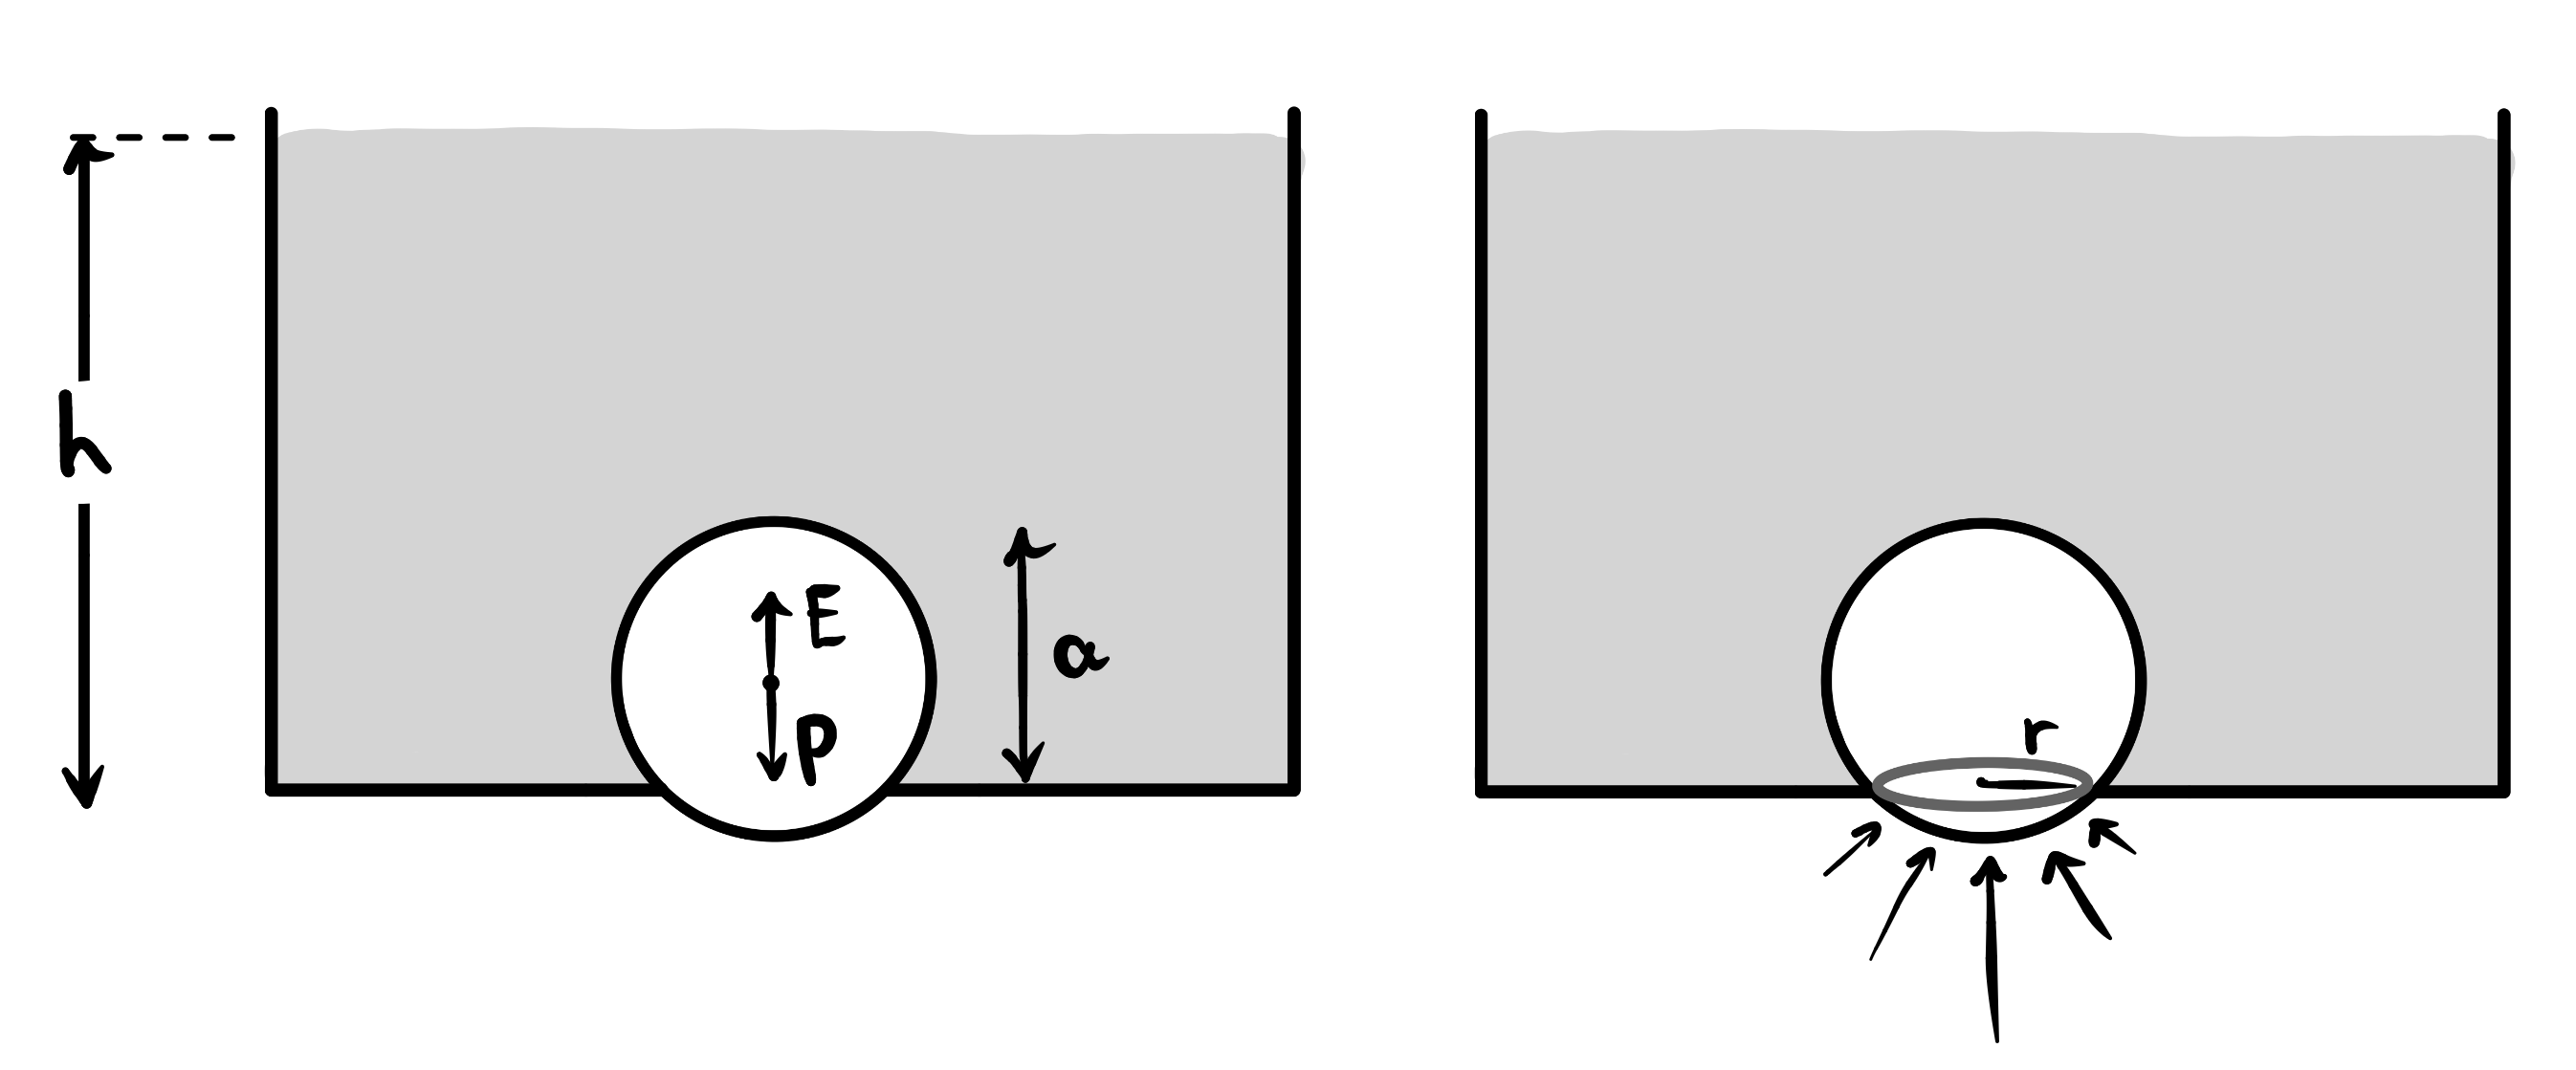
\includegraphics[width=0.65\linewidth]{imagensfluidos/empuxonaoarquiita2014.png}};
  \end{scope}
\end{tikzpicture}
\captionof{figure}{}
\label{fig_fluidos_empuxonaoarquiita2014}
} 
\vspace{0.3cm}


Assim, o empuxo que a bola sente, descontando a parcela que não atua, pelo fato do fundo da bola não estar em contato com o fluido, é:

$$ E = \rho V_D g - F =   \rho V_D g - \rho gh \pi r^2,$$

\noindent em que $V_D$ é o volume da bola imersa na água. Note que a expressão acima mostra porque, ao diminuir o nível $h$ da piscina, o empuxo \emph{aumenta:} a parcela subtraída cresce com $h$, de modo que diminuir $h$ diminui o tamanho da parcela subtraída, aumentando, portanto, o valor de $E.$ Assim, é possível diminuir o nível da água até que o empuxo se iguale com o peso da bolinha, permitindo que ela se desprenda do fundo, justamente como queremos. 

O volume de uma calota esférica -- que é volume da bola submerso -- é dado por

$$ V_D = \dfrac{\pi a}{6}(3r^2+a^2),$$

\noindent de modo que, na relação anterior, teremos:

$$ E = P \implies   \rho V_D g - \rho gh \pi r^2 = mg \implies   \rho \dfrac{\pi a}{6}(3r^2+a^2) \cancel  g - \rho \cancel gh \pi r^2 = m \cancel g, $$

\noindent de onde tiramos a altura $h$ em questão:

$$ \boxed{h = \dfrac{a}{6r^2}(3r^2+ a^2) - \dfrac{m}{\rho \pi r^2} \implies \text{letra E}.}$$





\end{exemplo}


\vspace{0.3cm}






\begin{secnivel}[Princípio de Pascal]{I}{Princípio de Pascal}
  
  \eqLdois{exp}{eq_fluidos_pascal}{\dfrac{F_1}{F_2} = \dfrac{A_1}{A_2}.}

\end{secnivel}





\secgfe{De onde vem}

Blaise Pascal nasceu em 1623, numa França que ainda se assombrava com as ideias de seu compatriota Descartes. Matemático prodígio -- autor, aos dezesseis anos, de um tratado de geometria projetiva que Descartes se recusou a acreditar que havia sido escrito por um adolescente --, Pascal dedicou parte de sua vida adulta ao estudo dos fluidos. O resultado mais duradouro dessa dedicação ficou conhecido como o Princípio de Pascal, enunciado em seu \textit{Traité de l'équilibre des liqueurs} (1663, publicado postumamente): uma pressão exercida sobre um fluido em repouso e confinado se transmite integralmente, sem perda, a todos os pontos desse fluido e às paredes do recipiente que o contém.


Imagine um recipiente fechado, completamente preenchido por um líquido incompressível, como o da Figura \ref{fig_fluidos_pascal}. Sobre esse líquido, aplica-se uma força $F_1$ em uma pequena área $A_1$ -- digamos, um êmbolo estreito do lado esquerdo. O que acontece com o restante do fluido?


\vspace{0.3cm}
{
\centering
\begin{tikzpicture}
  \begin{scope}[blend mode=multiply]
    \node {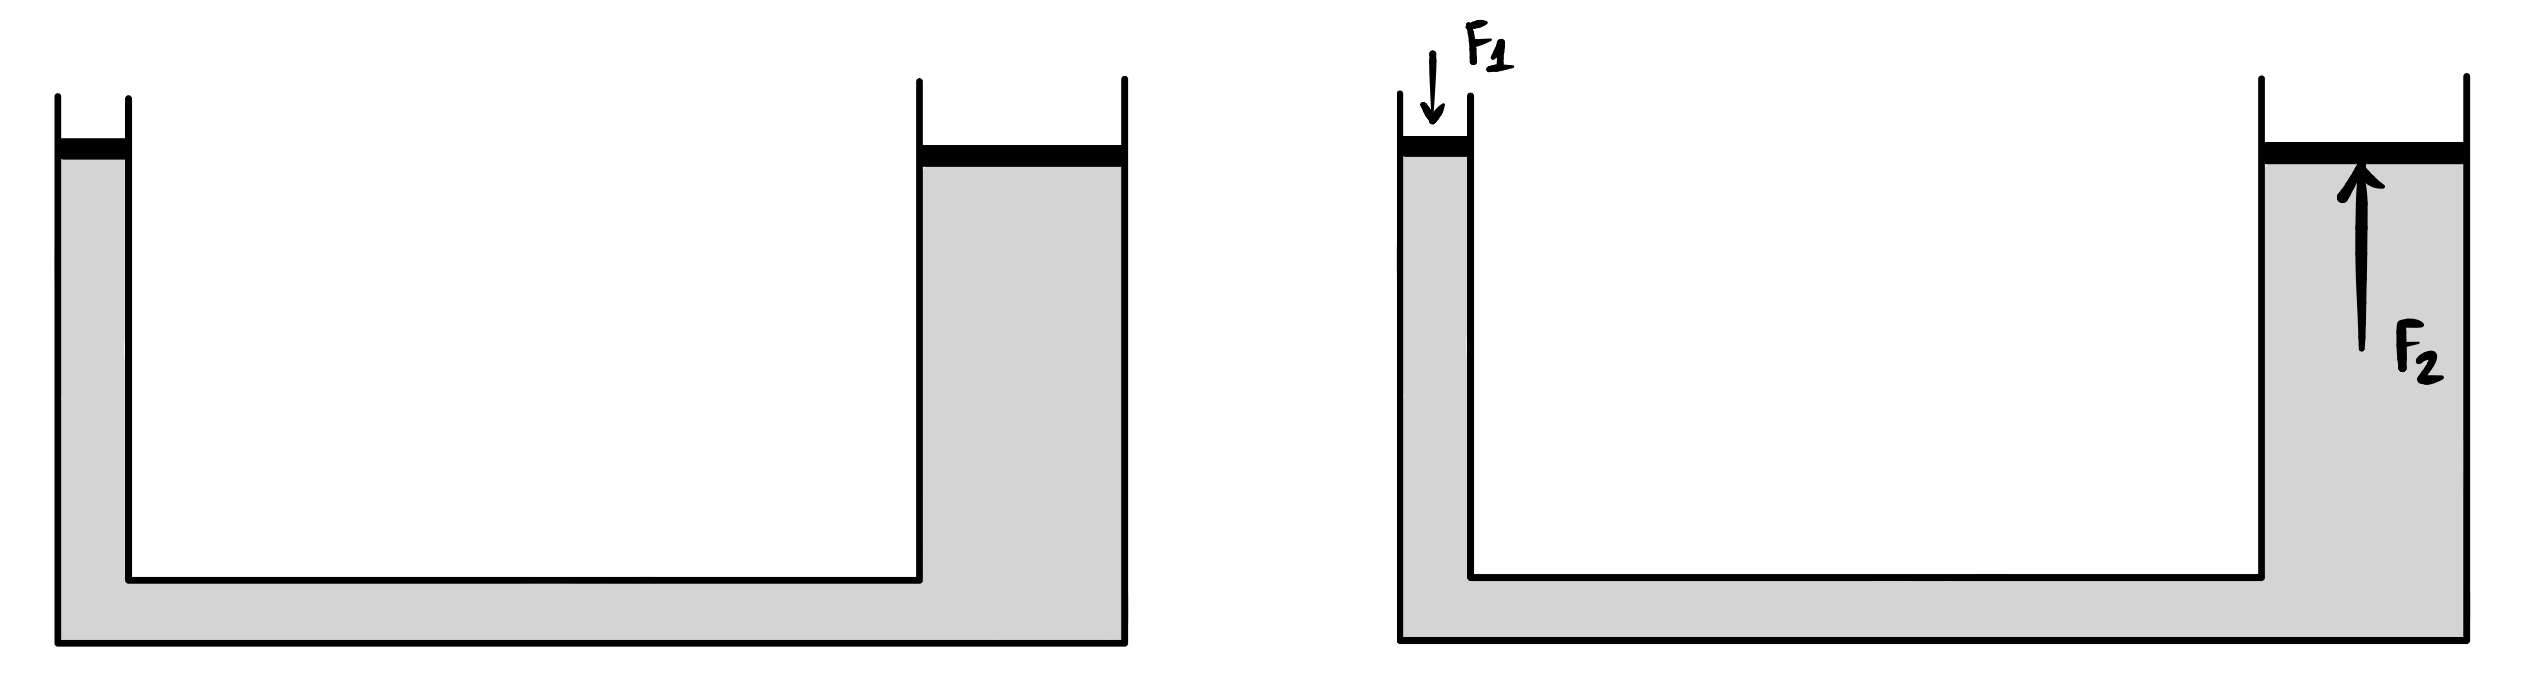
\includegraphics[width=0.75\linewidth]{imagensfluidos/pascal.png}};
  \end{scope}
\end{tikzpicture}
\captionof{figure}{O princípio de Pascal e os sistemas hidráulicos.}
\label{fig_fluidos_pascal}
} 
\vspace{0.3cm}




A observação experimental de Pascal -- e de muitos que o precederam, como Galileu e Torricelli -- é que a \emph{variação de pressão} gerada naquele ponto se propaga em todas as direções, com o mesmo valor, até cada centímetro quadrado das paredes e de qualquer outro êmbolo que exista no sistema. Se, do lado direito, há um segundo êmbolo de área $A_2$, a pressão que chega até ele é idêntica à que foi criada no primeiro:

\begin{equation}
   P_1 =  P_2
\end{equation}

Substituindo a definição de pressão em cada lado:

\begin{equation}
    \frac{F_1}{A_1} = \frac{F_2}{A_2},
\end{equation}

\noindent que pode ser reescrita no formato da Equação \eqref{eq_fluidos_pascal}. Perceba que, quanto maior for a área $A_2,$ maior terá que ser a força $F_2$ de modo que a razão entre elas forneça sempre o mesmo valor que $F_1/A_1$. Desse modo, podemos criar um sistema multiplicador de forças, semelhante ao que é feito com polias móveis, como vimos na Equação \eqref{eq_newton_poliamovel}.

Note que tal equação não é derivada matematicamente de um princípio mais profundo; ela é uma \textbf{lei experimental}, destilada da observação de que fluidos incompressíveis confinados se comportam dessa forma. A matemática aqui apenas organiza a observação de que a variação de pressão se transmite de forma integral a todos os pontos do fluido.

Mas por que o fluido transmite a pressão igualmente em todas as direções? A resposta está na própria natureza dos líquidos: ao contrário dos sólidos, cujas moléculas estão fixas em posições cristalinas, as moléculas de um líquido estão livres para se mover. Quando uma força comprime uma pequena região do fluido, as moléculas ali perturbadas empurram as vizinhas em todas as direções -- para cima, para baixo, para os lados -- que empurram as suas vizinhas, e assim por diante. O fluido age, em linguagem moderna, como um \textit{transmissor isotrópico de pressão}: não privilegia nenhuma direção.

% É importante notar que o Princípio de Pascal, nessa formulação ``pura'', ignora a variação de pressão com a profundidade que estudamos pela Lei de Stevin. Isso é razoável quando as dimensões do sistema são pequenas o suficiente para que a diferença de altura entre os êmbolos seja desprezível. Quando as alturas importam, o princípio deve ser combinado com a Lei de Stevin -- e voltaremos a isso nas Observações.

Sobre como este fato foi obtido experimentalmente, é interessante conhecer o experimento do barril de Pascal. O cientista tomou um barril de madeira robusto -- do tipo usado para armazenar vinho, com aduelas reforçadas por arcos de ferro -- e o encheu completamente com água. No topo do barril, inseriu um tubo fino e longo, de alguns milímetros de diâmetro interno, que se estendia verticalmente por cerca de dez metros de altura (alguns relatos históricos falam em um tubo fixado à fachada de um edifício). O barril foi hermeticamente vedado ao redor do tubo.


\vspace{0.3cm}
{
\centering
\begin{tikzpicture}
  \begin{scope}[blend mode=multiply]
    \node {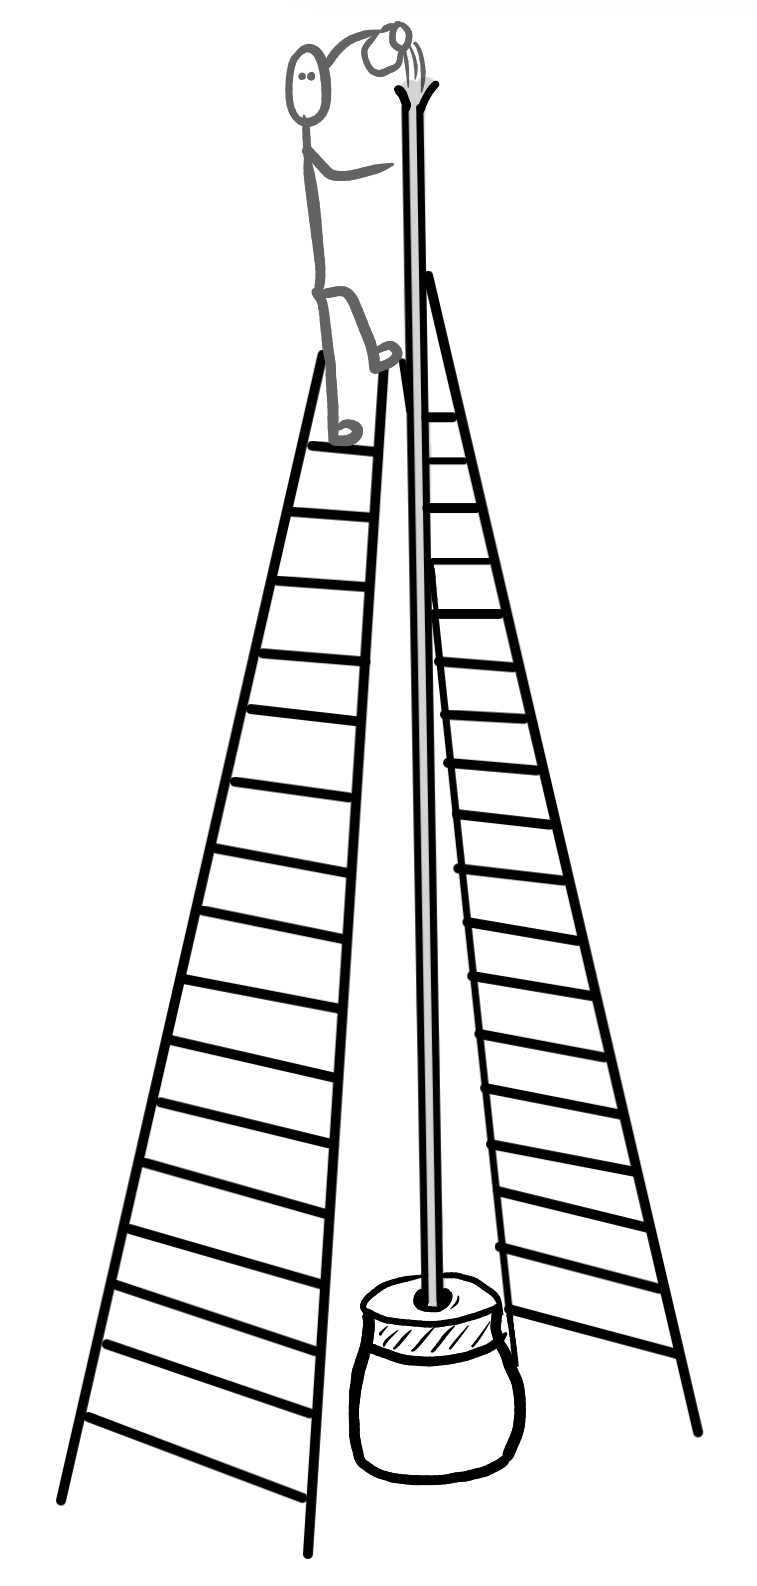
\includegraphics[width=0.25\linewidth]{imagensfluidos/pascalbarril.png}};
  \end{scope}
\end{tikzpicture}
\captionof{figure}{O experimento do barril de Pascal.}
\label{fig_fluidos_pascalbarril}
} 
\vspace{0.3cm}




O experimento era, em aparência, despretensioso. Pascal subiu ao andar superior com um pequeno jarro d'água e despejou uma quantidade modesta pelo topo do tubo. O volume adicionado era ínfimo -- algumas centenas de mililitros, no máximo. Mas a coluna de água de dez metros de altura gerou, na base do tubo, uma pressão de aproximadamente $1 \cdot 10^5 \text{ Pa} \approx 1 \text{ atm,}$ conforme já calculamos usando a Equação \eqref{eq_fluidos_leidestevin}. Esta pressão, transmitida integralmente a toda a superfície interna do barril, produziu uma força de vários milhares de newtons sobre as aduelas. O barril se estilhaçou.

A demonstração era clara: a força que destruiu o barril não vinha do jarro de água, cujo peso era irrisório. Vinha da pressão, amplificada pela grande área interna do recipiente. Pascal havia demonstrado, em público e de forma irrefutável, que a variação de pressão se transmite integralmente em todas as direções em um fluido confinado.

% O experimento é registrado no \emph{Traité de l'équilibre des liqueurs}, publicado postumamente em 1663, um ano após a morte de Pascal aos 39 anos. O texto original descreve o raciocínio com precisão notável para a época, sem dispor das ferramentas matemáticas que Euler e Cauchy desenvolveriam um século depois. Pascal operava com geometria e com uma intuição física de rara acuidade — e o barril estilhaçado foi seu argumento mais eloquente.



\secgfe{Onde é usada}

A Equação \eqref{eq_fluidos_pascal} é o coração dos sistemas hidráulicos. O sistema da Figura \ref{fig_fluidos_pascal} é exatamente o de um macaco hidráulico, presente em oficinas mecânicas. No êmbolo de maior área, $A_2,$ no caso, coloca-se um carro. Digamos que a sua massa é de 600 kg e a área de tal êmbolo é $A_2 = 9$m$^2$. Do lado esquerdo, tem-se um êmbolo de área $A_1 = 100 $ cm$^2$. Qual é a força $F_1$ que um mecânico deve fazer em tal êmbolo para erguer o carro?

Pela Equação \eqref{eq_fluidos_pascal}, teremos:

$$ \dfrac{F_1}{F_2} = \dfrac{A_1}{A_2} \implies \dfrac{F_1}{6.000 \text{ N}} = \dfrac{100 \text{ cm}^2}{90.000 \text{ cm}^2} 
\implies  \boxed{F_1 \approx 6.67\text{ N},} $$

\noindent ou seja, com uma força muito pequena é possível erguer objetos extremamente pesados. Esse é o princípio fundamental por trás de mecanismos hidráulicos. O mesmo ocorre em freios hidráulicos, presentes em carros modernos. Neles, a força do pé do motorista sobre o pedal é transmitida pelo fluido de freio até as pastilhas, que exercem força sobre os discos de cada roda. A geometria do sistema é projetada para que a força resultante nos freios seja muitas vezes maior que a força aplicada ao pedal. Prensas hidráulicas industriais também usam este princípio.



\secgfe{Erros comuns}

A Equação \eqref{eq_fluidos_pascal} é bem simples, não deixando muito espaço para erros. Cabe comentar aqui um erro -- mais de matemática do que de física, diga-se de passagem -- que acaba sendo recorrente entre os estudantes menos atentos.

Considere, como na situação da Figura \ref{fig_fluidos_pascal}, que temos dois êmbolos cilíndricos, de raios $r_1 = 2$m e $r_2 = 6$m. Qual é a razão entre as forças $F_2$ e $F_1?$

Em um primeiro momento, é comum que o leitor perceba que $r_2/r_1 = 6/2 = 3$ e, sendo o raio do êmbolo 2 o triplo do raio do êmbolo 1, conclui-se que a força $F_2$ em tal êmbolo será o triplo da força $F_1$ no primeiro êmbolo, isto é, $F_2 = 3F_1.$ 

O erro aqui consiste em ignorar que a razão entre as forças é igual à razão entre as \textbf{áreas} dos êmbolos e, para um êmbolo de área de seção transversal circular, sua área é $A= \pi r^2$. Ou seja, a razão entre as forças seria:

$$ \dfrac{F_1}{F_2} = \dfrac{A_1}{A_2} \implies  \dfrac{F_1}{F_2} = \dfrac{\cancel\pi r_1^2}{\cancel \pi r_2^2} \implies \boxed{ \dfrac{F_1}{F_2} =\left( \dfrac{r_1}{r_2} \right)^2 ,}$$

\noindent isto é, razão entre as forças não é igual à razão entre os raios, mas sim igual ao quadrado da razão entre os raios. Neste caso, $F_2/F_1 = 3^2 = 9.$

\secgfe{Observações}

Em um primeiro momento, tal como no estudo da polia móvel, o leitor pode estranhar um sistema multiplicador de forças. Isso, contudo, é perfeitamente possível -- não viola nenhuma lei da Física. Averiguemos isso. Considere a Figura \ref{fig_fluidos_pascalconservationofenergy}, em que aplicar-se-á uma força $F_1$ no êmbolo de área $A_1$, ao longo da distância $\Delta x_1.$ Isso irá gerar uma força $F_2$ no êmbolo de área $A_2,$ e um deslocamento $\Delta x_2$ de tal êmbolo.

\vspace{0.3cm}
{
\centering
\begin{tikzpicture}
  \begin{scope}[blend mode=multiply]
    \node {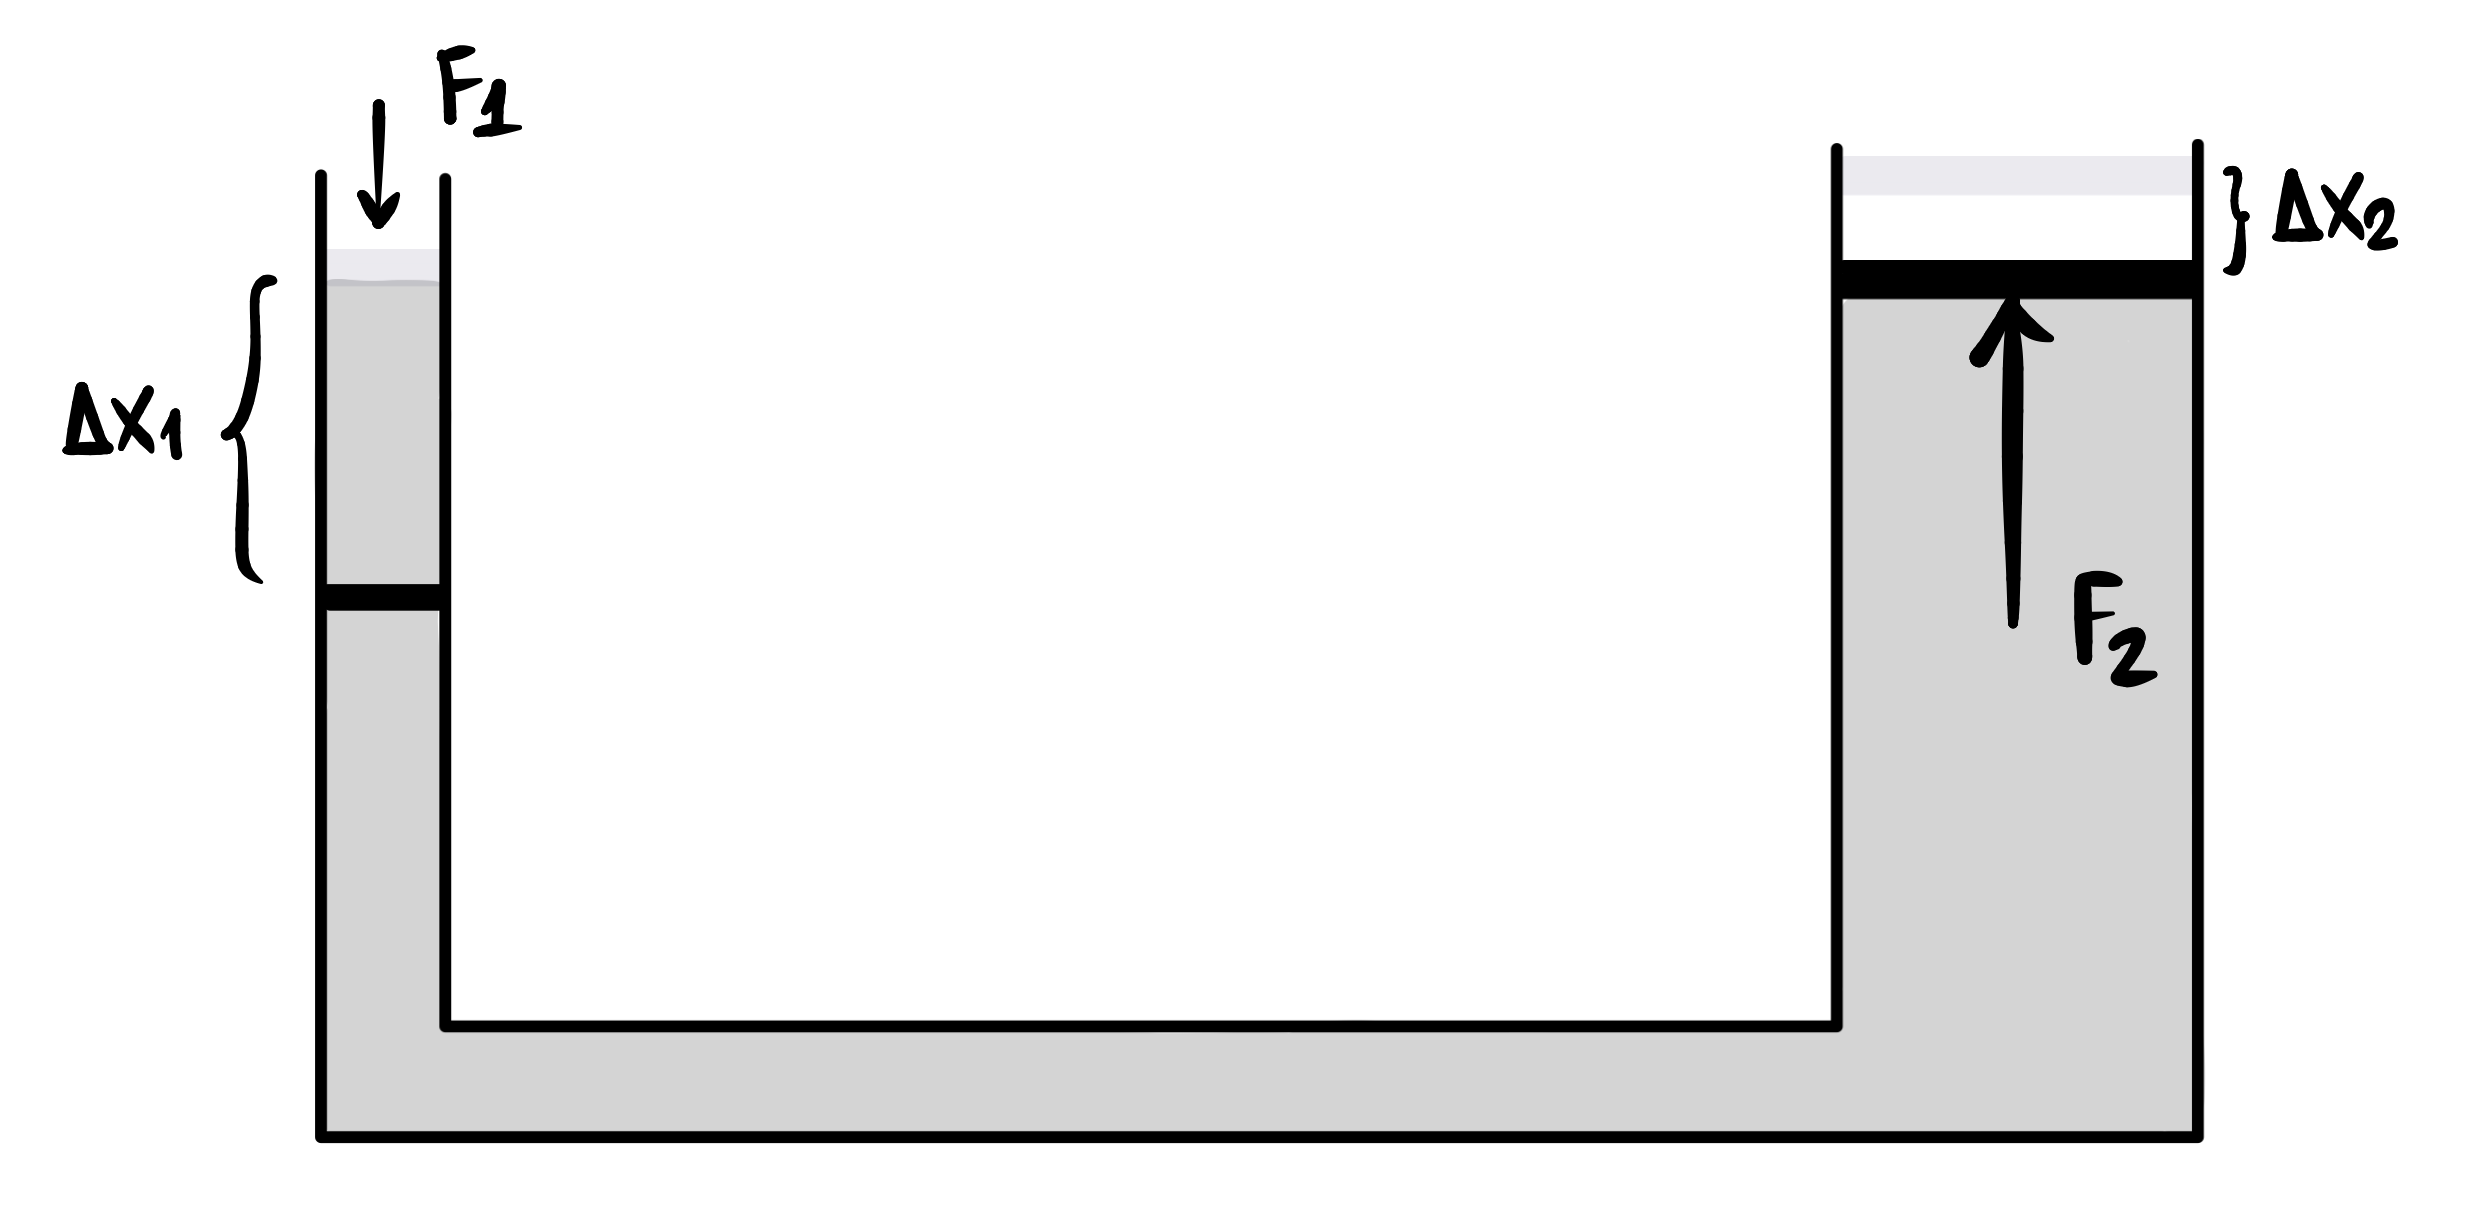
\includegraphics[width=0.5\linewidth]{imagensfluidos/pascalconservationofenergy.png}};
  \end{scope}
\end{tikzpicture}
\captionof{figure}{O sistema hidráulico e a conservação da energia.}
\label{fig_fluidos_pascalconservationofenergy}
} 
\vspace{0.3cm}


O volume líquido $A_1 \Delta x_1$ deslocado do lado esquerdo deve ser o mesmo que aparece do lado direito, isto é:

$$ A_1 \Delta x_1 = A_2 \Delta x_2,$$

\noindent ou seja, teremos

$$ \dfrac{A_1}{A_2}  = \dfrac{\Delta x_2}{\Delta x_1}.$$

Contudo, pelo princípio de Pascal, podemos escrever

$$ \dfrac{A_1}{A_2}  =  \dfrac{F_1}{F_2} =  \dfrac{\Delta x_2}{\Delta x_1} \implies F_1 \Delta x_1 = F_2 \Delta x_2 ,$$

\noindent ou seja, o trabalho $W_1 =F_1 \Delta x_1 $ impresso pela força $F_1$ de um lado deve ser exatamente igual ao trabalho $W_2 =F_2 \Delta x_2 $ da força $F_2$ empurrando o êmbolo do outro lado, o que garante a conservação da energia. Logo, vemos que o Princípio de Pascal, não violando a lei de conservação da energia, é um mecanismo fisicamente possível de multiplicar forças, tal e qual a polia móvel.

O preço que se paga, como naquele caso, é o de fazer deslocamentos maiores. Se o sistema multiplica a força por 10 e deseja-se erguer um objeto pesado de $\Delta x_2 =1 $m  de altura, seria preciso empurrar o êmbolo no lado de menor área de $\Delta x_1 = 10$m a fim de que isso fosse possível, haja vista que $F_1 \Delta x_1 = F_2 \Delta x_2.$




\vspace{0.3cm}

\begin{exemplo}[Nível I]\label{exemplo_fluidos_pascalex01}


Um sistema hidráulico industrial possui dois êmbolos circulares. O
êmbolo de entrada tem raio $r_1 = 3\ \text{cm}$ e o de saída tem raio
$r_2 = 15\ \text{cm}$. Uma força $F_1 = 400\ \text{N}$ é aplicada sobre
o êmbolo menor. Considerando os êmbolos à mesma altura e o fluido
incompressível, quanto vale a força exercida pelo êmbolo maior?

\resolucao

A área de um êmbolo circular de raio $r$ é $A = \pi r^2$. A razão entre
as áreas dos dois êmbolos é, portanto:

\begin{equation}
    \frac{A_2}{A_1} \nonumber
    = \frac{\pi r_2^2}{\pi r_1^2}
    = \left(\frac{r_2}{r_1}\right)^{\!2}
    = \left(\frac{15}{3}\right)^{\!2}
    = 5^2
    = 25
\end{equation}

Pelo Princípio de Pascal:

\begin{equation}
    \frac{F_1}{A_1} = \frac{F_2}{A_2} \nonumber
    \implies
    F_2 = F_1 \cdot \frac{A_2}{A_1} = 400 \cdot 25
    = 10.000\ \text{N}.
\end{equation}

\end{exemplo}

\vspace{0.3cm}






\begin{exemplo}[Nível II]\label{exemplo_fluidos_pascalex02}

Um sistema hidráulico tem êmbolo de entrada com área $A_1 = 10\ \text{cm}^2$
e êmbolo de saída com área $A_2 = 80\ \text{cm}^2$, ambos à mesma altura.
Uma caixa de massa $m = 48\ \text{kg}$ repousa sobre o êmbolo de saída.
O êmbolo de entrada é empurrado $d_1 = 80\ \text{cm}$ para baixo em um
único golpe. Considere $g = 10\ \text{m/s}^2$ e o fluido incompressível.
Quanto vale o trabalho realizado pelo sistema sobre a caixa durante esse deslocamento?


\resolucao


A força que o êmbolo de saída deve exercer sobre a caixa para que ela seja erguida deve ser pelo menos igual ao  seu peso:
\begin{equation}
    F_2 = mg = 48 \cdot 10 = 480\ \text{N} \nonumber 
\end{equation}


Como o fluido é incompressível, o volume varrido pelos dois êmbolos é
igual:
\begin{equation}
    A_1\, d_1 = A_2\, d_2 \nonumber 
    \implies
    d_2 = d_1 \cdot \frac{A_1}{A_2}
        = 80 \cdot \frac{10}{80}
        = 10\ \text{cm}
        = 0{,}10\ \text{m}
\end{equation}

O trabalho sob a caixa, portanto, pode ser computado por
\begin{equation}
    W = F_2 \cdot d_2 = 480 \cdot 0{,}10 = 48\ \text{J}. \nonumber 
\end{equation}

Verificando pela energia injetada na entrada, a força aplicada ao êmbolo de entrada segue do Princípio de Pascal:
\begin{equation}
    F_1 = F_2 \cdot \frac{A_1}{A_2} = 480 \cdot \frac{10}{80} = 60\ \text{N} \nonumber 
\end{equation}

O trabalho de entrada é $W = F_1 \cdot d_1 = 60 \cdot 0{,}80 = 48\ \text{J}$. Os dois resultados coincidem, confirmando a conservação de energia, como esperado.

\end{exemplo}



\vspace{0.3cm}







\begin{exemplo}[Nível III]\label{exemplo_fluidos_pascalex03}

Dois êmbolos de áreas $A_1$ (inferior) e $A_2$ (superior) estão
conectados por um fluido de densidade $\rho$. A diferença de altura entre
eles é $h$ ($A_2$ está acima de $A_1$). Uma força $F_1$ é aplicada sobre
o êmbolo inferior. Expresse a força $F_2$ exercida pelo êmbolo superior
em função de $F_1$, $A_1$, $A_2$, $\rho$, $g$ e $h$.


\resolucao

A pressão produzida pelo êmbolo inferior sobre o fluido é:
\begin{equation}
    P_1 = \frac{F_1}{A_1} \nonumber
\end{equation}

Como o êmbolo superior está a uma altura $h$ acima do inferior, a pressão
que o fluido exerce \emph{sobre ele} é menor do que $P_1$. Pela Lei de
Stevin, a pressão decresce com a altura segundo $\rho g h$ por metro
ascendido. Portanto:
\begin{equation}
    P_2 = P_1 - \rho g h = \frac{F_1}{A_1} - \rho g h \nonumber
\end{equation} 

A força resultante sobre o êmbolo superior é pressão vezes área:
\begin{equation}
    \boxed{F_2 = P_2 \cdot A_2 = A_2\!\left(\frac{F_1}{A_1} - \rho g h\right)} \nonumber
\end{equation}

Note que $F_2 < F_1 \cdot A_2/A_1$: a diferença de altura \emph{reduz}
a força disponível no êmbolo superior, pois parte da energia da pressão
aplicada é consumida para sustentar a coluna de fluido de altura $h$.
Apenas quando $h = 0$ a expressão se reduz ao Pascal puro,
$F_2 = F_1 A_2/A_1$.


\end{exemplo}



\vspace{0.3cm}









% \section{Hidrodinâmica}





% \begin{secnivel}{I}{Vazão}
  
%   \eqLdois{def}{eq_fluidos_hidrodinamicavazao}{\phi = \dfrac{\Delta V}{\Delta t}}

% \end{secnivel}







% \secgfe{De onde vem}



% \secgfe{Onde é usada}



% \secgfe{Erros comuns}




% \secgfe{Observações}



% \vspace{0.3cm}


% \begin{exemplo}[Nível I]\label{exemplo_fluidos_hidrodinamicavazaoex01}


% \resolucao


% \end{exemplo}




% \vspace{0.3cm}


% \begin{exemplo}[Nível II]\label{exemplo_fluidos_hidrodinamicavazaoex02}


% \resolucao


% \end{exemplo}


% \vspace{0.3cm}










% \begin{secnivel}{II}{Equação da Continuidade}
  
%   \eqLdois{dem}{eq_fluidos_hidrodinamicacontinuidade}{A_1v_1=A_2v_2}

% \end{secnivel}










% \secgfe{De onde vem}



% \secgfe{Onde é usada}



% \secgfe{Erros comuns}




% \secgfe{Observações}



% \vspace{0.3cm}


% \begin{exemplo}[Nível I]\label{exemplo_fluidos_hidrodinamicacontinuidadeex01}


% \resolucao


% \end{exemplo}


% \vspace{0.3cm}




% \begin{exemplo}[Nível II]\label{exemplo_fluidos_hidrodinamicacontinuidadeex02}


% \resolucao


% \end{exemplo}




% \vspace{0.3cm}





% \begin{exemplo}[Nível III]\label{exemplo_fluidos_hidrodinamicacontinuidadeex03}


% \resolucao


% \end{exemplo}




% \vspace{0.3cm}









% \begin{secnivel}{III}{Equação de Bernoulli}
  
%   \eqLdois{dem}{eq_fluidos_hidrodinamicabernoulli}{P_1 + \rho gh_1 + \dfrac{1}{2}\rho v_1^2 = P_2 + \rho gh_2 + \dfrac{1}{2}\rho v_2^2}

% \end{secnivel}









% \secgfe{De onde vem}



% \secgfe{Onde é usada}



% \secgfe{Erros comuns}




% \secgfe{Observações}


% \vspace{0.3cm}


% \begin{exemplo}[Nível III]\label{exemplo_fluidos_hidrodinamicabernoulliex01}

% Princípio de bernoulli

% \resolucao


% \end{exemplo}

% \vspace{0.3cm}






% \begin{exemplo}[Nível III]\label{exemplo_fluidos_hidrodinamicabernoulliex02}


% tubo de pitot

% \resolucao


% \end{exemplo}


% \vspace{0.3cm}


% \begin{exemplo}[Nível III]\label{exemplo_fluidos_hidrodinamicabernoulliex03}


% tubo de venturi

% \resolucao


% \end{exemplo}






